\chapter{Modelli generativi di grafi aleatori e loro rilevanza nella rappresentazione di reti}

In questo primo capitolo ci focalizzeremo sulla nozione di "inventare" una rete. Un modo intuitivo e semplice di "inventare" una rete, consiste nel generare un grafo in modo casuale. Ossia, generare un grafo in cui gli archi fra i nodi sono scelti sulla base di un evento aleatorio. Esistono diversi modelli per generare grafi casuali, ovvero delle regole probabilistiche che permettono di connettere nodi. Il primo modello che andremo ad analizzare è quello di Erd\"{o}s-Renyi. 

\section{Il Modello di Erd\"{o}s-Renyi}

\begin{definizione}[Modello di Erd\"{o}s-Renyi]
    Fissati $n \in \mathbb{N}$ e $p \in [0,1]$. Definiamo il \textbf{grafo aleatorio $G_{n,p} = \{V_{n,p},\ E_{n,p}\}$}, il grafo costruito a partire da $n$ e $p$ nel seguente modo:
    \begin{itemize}
        \item $V_{n,p} = [n] = \{1, 2, 3, \dots, n\}$ è l'insieme dei nodi;
        \item $E_{n, p} = \{(i, j): i,j \in V_{n_p} \land i \neq j\ |\ \Pr[(i, j) \in E_{n, p}] = p\}$
    \end{itemize}
\end{definizione}

 In altre parole, presi due nodi distinti $i, j \in V_{n,p}$, allora con probabilità $p$, l'arco $(i, j) \in E_{n, p}$, mentre con probabilità $1 - p$, l'arco $(i, j) \notin E_{n, p}$.

Definito il modello di generazione del grafo, quello che interezza studiare ora è l'esistenza di una componente gigante e il grado dei nodi. Osserviamo inanzi tutto, che, fissato il numero $n$ di nodi, al variare di $p$ otterremo grafi con caratteristiche molto differenti.

\begin{itemize}
    \item Se $p = 0$, allora $G_{n,0} = \{[n], \emptyset\}$, ovvero il grafo non contiene archi.
    \item Se $p = 1$, allora $G_{n, 1}$ è il grafo completo su $n$ nodi, ovvero $|E_{n,1}| = \binom{n}{2} = \frac{n(n - 1)}{2}$.
\end{itemize}

 Nelle prossime sezioni andremo quindi a quantificare le seguenti proprietà:
\begin{itemize}[label={-}]
    \item $G_{n,p}$ conterrà \textbf{mediamente} tanti più archi quanto più $p$ si avvicina a 1.
    \item \textbf{Mediamente}, un nodo avrà tanti più vicini quanto più $p$ si avvicina a 1.
    \item \textbf{Mediamente}, le componenti connesse di $G_{n,p}$ saranno tanto più grandi quanto più $p$ si avvicina a 1.
\end{itemize}

\subsection{Componenti Giganti}

\begin{definizione}[Componente Gigante]
    Una \textbf{componente gigante} in un grafo è una componente connessa che contiene \textit{una frazione del numero dei nodi}.
    
     Formalmente, in un grafo $G$ con $n$ nodi, si dice che esiste una \textbf{componente gigante} se c'è una componente connessa $C$ tale che la sua cardinalità $|C|$ è proporzionale a $n$ (cioè $|C| \approx n$ per $n \rightarrow \infty$).
\end{definizione}

\vspace{0.5cm}

 Molte reti reali contengono una componente gigante, come per esempio le reti sociali e, come vederemo più avanti, anche nella rete del Web.

La domanda alla quale vorremmo rispondere ora è: il modello di Erd\"os-Renyi riesce a rappresentare questa caratteristica di molte reti reali? Esistono quindi dei valori per $p$ tali che, il grafo $G_{n,p}$ contiene componenti giganti?

\begin{teorema}[Esistenza di Componenti Giganti]\label{theoem1.1}
    Sia $X$ la variabile aleatoria corrispondente al numero di nodi nella più grande componente connessa di $G_{n,p}$ e supponiamo che $p > \frac{\ln(64)}{n}$, allora,
    \[
    \Pr[X \geq \frac{n}{2}] \geq 1 - 2^{-\frac{n}{8}} = 1 - \frac{1}{2^{n/8}}
    \]
\end{teorema}

 In altre parole, se $p > \frac{\ln(64)}{n}$, allora \textbf{con alta probabilità}\footnote{Con alta probabilità si intende una probabilità proporzionale almeno a $1 - \frac{b}{n^c}$, per qualche coppia di costanti positive $b$ e $c$.} $G_{n,p}$ contiene una componente connessa costituita da almeno metà dei suoi nodi.
    
 Per dimostrare il teorema appena enunciato abbiamo bisogno del seguente lemma:

\begin{lemma}\label{lemma1.2}
    Se $X < \frac{n}{2}$, allora esiste un insieme $A \subset [n]$ tale che
    \begin{itemize}
        \item $\frac{n}{4} \leq |A| < \frac{3n}{4}$
        \item $\forall i \in A, \forall j \in [n] \setminus A, (i, j) \notin E_{n,p}$ - non esistono archi fra i nodi in $A$ e i nodi in $[n] \setminus A$.
    \end{itemize}
    
    \begin{proof}
        Siano $C_1, C_2, \dots, C_k$ tutte le componenti connesse di $G_{n,p}$ e assumiamo che siano ordinate per cardinalità non decrescente, ossia $|C_1|, \leq |C_2|, \leq \dots, \leq |C_k|$.
        
         Poiché $X < \frac{n}{2}$, allora $|C_i| < \frac{n}{2},\ \forall\ i=1, \dots, k$, scegliamo un indice $h$ tale che: 
        \[
        \begin{aligned}
        & |C_1| + |C_2|+ \dots+ |C_{h-1}| < \frac{n}{4} \\ 
        & \land\\
        & |C_1| + |C_2|+ \dots+ |C_{h-1}| + |C_h| \geq \frac{n}{4}
        \end{aligned}
        \]
        Notiamo inoltre che $h < k$, in quanto se fosse $h = k$, sapendo che $|C_k| < \frac{n}{2}$ risulterebbe:
        \[
        |C_1| + |C_2|+ \dots+ |C_{k-1}| + |C_k| < \frac{n}{4} + \frac{n}{2} < n
        \]
        che è impossibile dato che la somma delle cardinalità di tutte le componenti deve essere proprio $n$.
        A questo punto, \textbf{scegliamo} $A = C_1 \cup C_2 \cup \dots \cup C_h$, osservando quindi che $A \neq \emptyset$ e $[n] \setminus A = C_{h+1} \cup C_2 \cup \dots \cup C_k \neq \emptyset$.
        
         Ovviamente,
        \begin{itemize}
            \item $|A| \geq \frac{n}{4}$, per costruzione
            \item $|A| = |C_1| + |C_2|+ \dots+ |C_{h-1}| + |C_h| < \frac{n}{4} + \frac{n}{2} = \frac{3n}{4}$
        \end{itemize}
        dimostrando il primo risultato.
        
         Rimane da dimostrare che non esistono archi tra $A$ e $[n] \setminus A$. Sempre per costruzione, poiché $C_1, C_2, \dots, C_k$ sono tutte le componenti connesse di $G_{n,p}$, non ci sono archi fra $A$ e $[n] \setminus A$ per definizione di componente connessa, in quanto, se ci fosse un arco fra $C_i$ e $C_j$ con $1 \leq i \leq h$ e $h < j \leq k$, allora $C_i \cup C_j$ sarebbe un'unica componente connessa.

         In conclusione, chiamiamo insieme \textbf{buono} l'insieme $A$ appena individuato.
    \end{proof}
\end{lemma}

\begin{osservazione}\label{osservazione1.1}
    Il \autoref{lemma1.2} ci assicura che \textit{la probabilità che la più grande componente connessa di $G_{n,p}$ contenga meno di $\frac{n}{2}$ nodi è minore o uguale alla probabilità che $G_{n,p}$ contenga un insieme di nodi buono}\footnote{Dati due eventi $e_1$ e $e_2$, se $e_1 \Rightarrow e_2$, allora $\Pr[e_1] \leq \Pr[e_2]$.}.
\end{osservazione}

\newpage

\begin{proof}[\autoref{theoem1.1}]
    Dimostreremo il teorema per assurdo. Supponiamo quindi di voler calcolare $\Pr[X < \frac{n}{2}]$, ossia la probabilità che la massima componente connessa di $G_{n,p}$ contenga meno di $\frac{n}{2}$ nodi (che è l'evento complementare dell'evento $X \geq \frac{n}{2}$ che ci interessa).
    In virtù all'\autoref{osservazione1.1}:

\begin{align*}
    \Pr\left[X < \frac{n}{2}\right] &\leq \Pr[\exists\ A \subset [n]: A \text{ è buono}] \\
    &= \Pr \left[\bigcup_{A \subset [n],\ \frac{n}{4} \leq |A| < \frac{3n}{4}} (\text{non ci sono archi fra $A$ e $[n] \setminus A$}) \right] \\
    &\leq \sum_{A \subset [n],\ \frac{n}{4} \leq |A| < \frac{3n}{4}} (\text{non ci sono archi fra $A$ e $[n] \setminus A$}) \\
    \intertext{Per la Union Bound.}
    &= \sum_{A \subset [n],\ \frac{n}{4} \leq |A| < \frac{3n}{4}} (1-p)^{|A|(n-|A|)} \\
    \intertext{\small Il numero di archi possibili fra $A$ e $[n] \setminus A$ è $|A| \cdot (n - |A|)$ con probabilità $(1 - p)$.}
    &\leq \sum_{A \subset [n],\ \frac{n}{4} \leq |A| < \frac{3n}{4}} (1-p)^{3n^2/16} \\
    \intertext{\small (Perché $(1 - p) < 1$, ossia $(1 - p)^z$ è massimo quando $z$ è minimo. Nel nostro caso, $|A|(n - |A|)$ è minimo per $|A| = n/4$ oppure per $|A| = 3n/4$) in quanto è una parabola.}
    &\leq 2^n (1-p)^{3n^2/16} \\
    \intertext{\small In quanto $[n]$ contiene al più $2^n$ sottoinsiemi.}
    &< 2^n \left(1 - \frac{\ln(64)}{n} \right)^{\frac{3n^2}{16}} \\
    \intertext{\small Usiamo l'ipotesi che $p > \frac{\ln(64)}{n}$, quindi si passa da $\leq$ a $<$.}
    &= 2^n \left[\left(1 - \frac{\ln(64)}{n} \right)^n\right]^{\frac{3n}{16}} \\
    \intertext{\small Moltiplichiamo e dividiamo l'esponente $n$ per $-\ln(64)$}
    &= 2^n \left[\left(1 - \frac{\ln(64)}{n} \right)^{\frac{-n}{\ln(64)}(-\ln(64))}\right]^{\frac{3n}{16}} \\
    \intertext{\small Poiché $\lim_{n \to \infty} (\left(1 - \frac{\ln(64)}{n} \right)^{\frac{-n}{\ln(64)}} = e$, allora $\left(1 - \frac{\ln(64)}{n} \right)^{\frac{-n}{\ln(64)}(-\ln(64))} \approx e^{-\ln(64)} = 64^{-1}$.}
\end{align*}
\[
\Pr[X < \frac{n}{2}] < 2^n [64^{-1}]^{3n/16} = 2^n [2^{-6}]^{3n/16} = 2^n 2^{-18n/16} = 2^{-n/8} 
\]
dimostrando quindi per assurdo il \autoref{theoem1.1}. 
\end{proof}

\begin{teorema}
    Al \autoref{theoem1.1}, si può dimostrare che:
    \begin{enumerate}
        \item Se $p(n - 1) < 1$, allora quasi sicuramente\footnote{"Quasi sicuramente" significa che, al tendere di $n$ all'infinito, la probabilità dell'evento tende a 1, un pò meno che con alta probabilità.} tutte le componenti connesse di $G_{n,p}$ hanno $O(\log n)$ nodi;
        \item Se $p(n - 1) = 1$, allora quasi sicuramente $G_{n,p}$ ha una componente connessa di $\approx n^{2/3}$ nodi;
        \item Se $p(n - 1) > 1$, allora quasi sicuramente $G_{n,p}$ ha una componente connessa di $\Omega(n)$ nodi e tutte le altre connesse hanno $O(\log n)$ nodi.
    \end{enumerate}
\end{teorema}

 In conclusione, la presenza di componenti giganti dipende dal prodotto $p(n - 1)$.

\subsection{Grado dei Nodi}

In questa parte andremo a capire meglio cosa rappresenta il prodotto $p(n - 1)$.

\begin{definizione}[Valore Atteso del Grado dei Nodi]
Sia $\delta_i$ la variabile aleatoria che esprime il grado del nodo $i$, ovvero:
\begin{align*}
    \delta_i &= \sum_{j \in [n] \setminus \{i\}} a_{ij}
\end{align*}
dove $a_{ij}$ è la variabile indicatrice che vale 1 se esiste l'arco $(i,j)$ e 0 altrimenti.

 Il valore atteso del grado del nodo $i$ in $G(n,p)$ è:
\begin{align*}
    \mathbb{E}[\delta_i] &= \mathbb{E}[\sum_{j \in [n] \setminus \{i\}} a_{ij}] \\
    &= \sum_{j \in [n] \setminus \{i\}} \mathbb{E}[a_{ij}] \\
    &= \sum_{j \in [n] \setminus \{i\}} [1 \cdot p + 0 \cdot (1 - p)] \\
    &= \sum_{j \in [n] \setminus \{i\}} p = (n - 1) p\\
\end{align*}
 Questo significa che, se $p$ è costante, il grado dei nodi, \textbf{in media}, cresce linearmente con il numero dei nodi. 
\end{definizione}

Questo però non è realistico, in quanto nelle reti sociali vere, non è detto che se la popolazione cresce, allora anche i "contatti" di un individuo crescono, quindi non è ragionevole per la modellizzazione delle reti sociali reali usare un $p$ costante, perché il grado medio diverrebbe molto grande per $p$ grande.
Per questa ragione, al fine di modellare significativamente reti reali di grandi
dimensioni è opportuno che $p$ sia una funzione decrescente di $n$, del tipo:
\[
p = p(n) = \frac{\lambda}{n}
\]
per qualche costante positiva $\lambda$.

\newpage

Dunque, fissato un intero $k < n$, vogliamo calcolare \textbf{con quale probabilità un nodo in $G_{n,p}$ ha grado $k$}.
Preso $i \in [n]$, la probabilità che il nodo $i$ abbia grado $k$ è la probabilità che \textbf{esattamente} $k$ altri nodi siano adiacenti a $i$, ovvero:
\begin{itemize}
    \item Il numero di possibili $k$-tuple di nodi scelti nell'insieme $[n] - \{i\} \text{ è } \binom{n-1}{k}$;
    \item La probabilià che vi sia un arco fra $i$ e \textbf{ciascuno} dei nodi della $k$-tupla è $p^k$;
    \item La probabilità che \textbf{non} vi sia un arco fra $i$ e \textbf{ciascuno} dei nodi non contenuto nella $k$-tupla è $(1-p)^{n-k-1}$.
\end{itemize}
Formalmente, vogliamo calcolare:
\begin{align*}
    \Pr[\delta_i = k] &= \binom{n - 1}{k}p^k(1-p)^{n-k-1} \\
    &= \binom{n - 1}{k}\frac{\lambda^k}{n^k}\left(1-\frac{\lambda}{n}\right)^{n-k-1} \\
    &= \frac{(n-1)(n-2)\dots(n-k)}{k!}\frac{\lambda^k}{n^k}\left(1-\frac{\lambda}{n}\right)^{n-k-1} \\
    &< \frac{(n-1)(n-2)\dots(n-k)}{k!}\frac{\lambda^k}{n^k} e^{\frac{-\lambda(n-k-1)}{n}} \\
    \intertext{\small $\forall x \in (0,1)$ vale che $(1-x) < e^{-x}$.}
    &< \frac{n^k}{k!}\frac{\lambda^k}{n^k} e^{\frac{-\lambda(n-k-1)}{n}} \approx \frac{n^k}{k!}\frac{\lambda^k}{n^k} e^{-\lambda} \\
    \intertext{per $n$ sufficientemente grande.}
\end{align*}
\begin{align*}
    \Pr[\delta_i = k] &< \frac{\lambda^k}{k!} e^{-\lambda} \\
    &\approx \frac{(\lambda e)^k}{\sqrt{2\pi k}\ k^k} e^{-\lambda} = \frac{e^{-\lambda}}{\sqrt{2\pi k}} \left(\frac{\lambda e}{k}\right)^k \\
    \intertext{\small sapendo che $k! \approx \sqrt{2\pi k}\left(\frac{k}{e}\right)^k$ - approssimazione di Stirling.}
\end{align*}

 Dunque, possiamo concludere che \textbf{la probabilità che un generico nodo abbia grado $k$} decresce molto velocemente al crescere di $k$, ovvero decresce come $k^{-k}$ (\textbf{decresce esponenzialmente in $k$}).

\newpage

Un'ulteriore domanda alla quale vogliamo rispondere è: \textbf{qual è la frazione del numero di nodi che hanno grado $k$?}

Definiamo $F_k$ la variabile aleatoria che esprime tale frazione e con $\delta_{ik}$ la variabile aleatoria che vale 1 se $\delta_i = k,\ 0$ altrimenti, allora:
\[
F_k = \frac{1}{n}\sum_{i \in [n]} \delta_{ik}
\]
Passando al valore atteso, abbiamo che:
\begin{align*}
    \mathbb{E}[F_k] &= \mathbb{E}\left[\frac{1}{n}\sum_{i \in [n]} \delta_{ik}\right] = \frac{1}{n}\sum_{i \in [n]} \mathbb{E}[\delta_{ik}] \\
    &= \frac{1}{n}\sum_{i \in [n]}[\Pr(\delta_{ik} = k)] \\
    &< \frac{e^{-\lambda}}{\sqrt{2\pi k}} \left(\frac{\lambda e}{k}\right)^k
\end{align*}

 Ossia, mediamente, la frazione del numero di nodi che hanno grado $k$ decresce come $k^{-k}$, ovvero \textbf{esponenzialmente in $k$}.

\newpage 

\section{Power Law, Rich Get Richer e Modello Barabasi-Albert}

Nel modello di Erd\"os-Renyi la porzione di grafo che già è stata costruita (gli archi che sono già stati inseriti in $G_{n,p}$) non ha alcuna influenza sul prossimo arco che verrà creato.

Consideriamo il grafo orientato del web: i nodi sono le pagine e, se la pagina $a$ contiene un hyperlink alla pagina $b$, allora $(a,b)$ è un arco diretto del grafo. Analizzando la distribuzione dei gradi (considerando solo gli archi entranti) nei nodi del grafo del web, si è osservato che differisce \textbf{sostanzialmente} da quanto indicato nel Teorema del Limite Centrale: \textbf{la frazione di pagine web che ha grado entrante $k$ è proporzionale a $\frac{1}{k^c}$ per qualche costante $c$, invece che a $\frac{1}{k^k}$}, risultato ottenuto nel capitolo precedente.

In altre parole, il numero di nodi del grafo del web che hanno grado entrante elevato è molto maggiore di quello che ci si aspetterebbe assumendo che gli archi si formino \textbf{indipendentemente} gli uni dagli altri.

 Una funzione che decresce come l'inverso di un polinomio è chiamata \textbf{power law}.

\subsection{Come riconoscere una Power Law?}

Invece di considerare il grafico vero della funzione, si considera il grafico $\log-\log$, ovvero un grafico i cui assi rappresentano $\ln(x)$ e $\ln(y)$, quindi invece di rappresentare $y = f(k)$, andremo a rappresentare $\ln(y) = \ln(f(k))$, dove con $f(k)$ indichiamo la funzione che esprime il numero di nodi di grado $k$. In questo modo, se $f(k) = \frac{1}{k^c}$, il grafo sarà, grosso modo una retta, ovvero $\ln(y) = -c\ln(k)$.

\begin{figure}[htbp]
    \centering
    \begin{subfigure}[t]{0.45\textwidth}
        \centering
        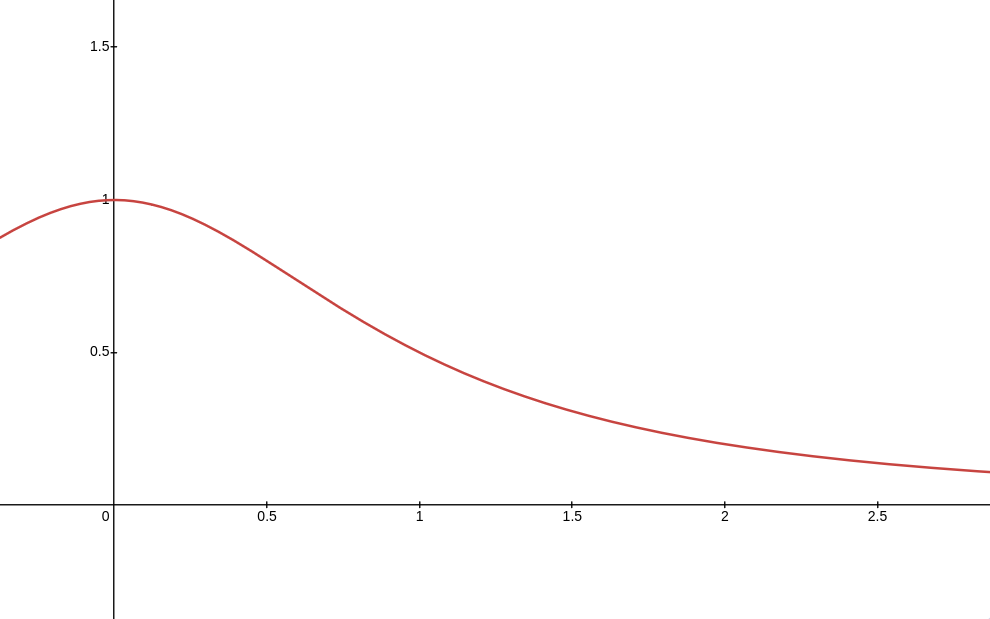
\includegraphics[width=\textwidth]{images/normalplot.png}
        \caption{Plot della funzione $f(x) = \frac{1}{x^2 + 1}$}
    \end{subfigure}
    \hfill
    \begin{subfigure}[t]{0.45\textwidth}
        \centering
        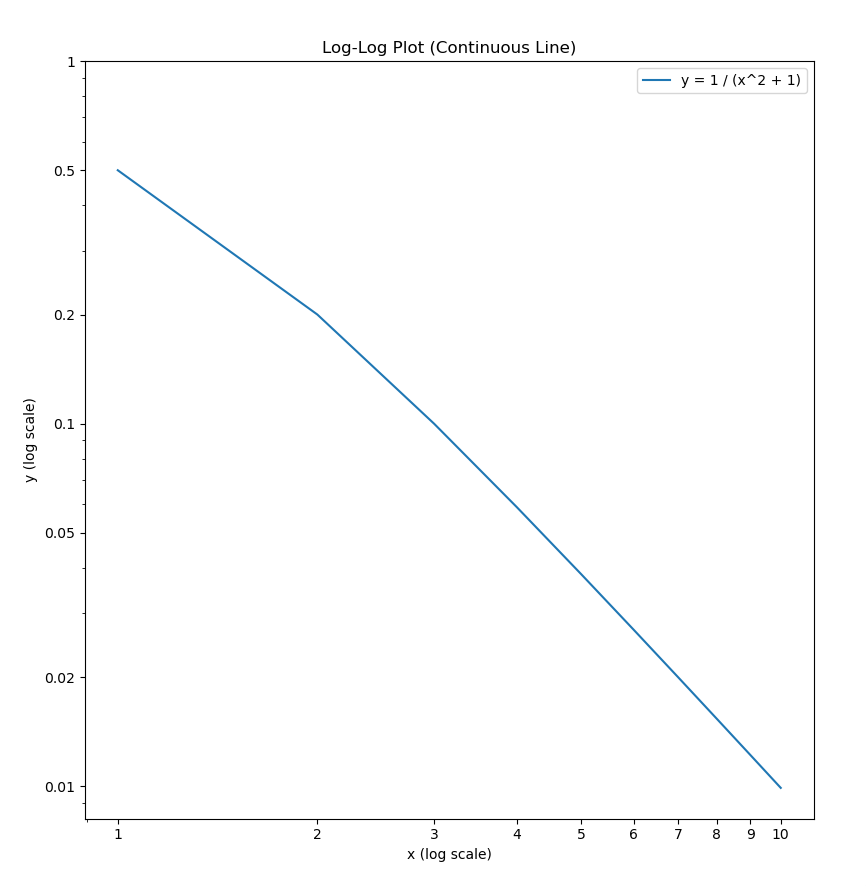
\includegraphics[width=\textwidth]{images/loglog.png}
        \caption{Plot della funzione $\ln(f(x)) = \ln\left(\frac{1}{x^2 + 1}\right)$}
    \end{subfigure}
    \label{fig:doppia}
\end{figure}

\subsection{Fenomeno Rich Get Richer}

 Il fenomeno "rich get richer" descrive una dinamica in cui chi ha già molte risorse o connessioni tende ad accumularne ancora di più, mentre chi parte svantaggiato resta indietro. Un esempio concreto si trova nella costruzione del grafo del web: quando crei una nuova pagina su un argomento, spesso inserisci un hyperlink verso una fonte autorevole trovata tramite motore di ricerca. La pagina che scegli di linkare è in cima ai risultati proprio perché ha già molti link entranti, quindi è considerata più autorevole. Così, aggiungendo il tuo link, contribuisci ad aumentare ulteriormente il grado di quella pagina già popolare. \textbf{In pratica, scegliamo quale arco aggiungere sulla base degli archi già presenti!}

\subsection{Modello Barabasi-Albert}

A questo punto vogliamo definire un modello di generazione di grafi aleatori che esprima il fenomeno "rich get richer", nel quale l'aggiunta di un nuovo arco dipenda dagli archi già presenti nel grafo, e che tale modello esibisca una power law.
\vspace{0.5cm}
\begin{definizione}[Modello Barabasi-Albert]
    Fissato $p \in [0, 1]$. Definiamo il grafo diretto $G_{p} = \{V_{p}, E_{p}\}$, il grafo aleatorio costruito nel seguente modo:
    \begin{enumerate}
        \item Al passo 1 viene creato il nodo 1: $V_{p,1} = \{1\}$;
        \item Al passo 2 viene creato il nodo 2: $V_{p,2} = \{1, 2\}$ e $E_{p,2} = \{(2, 1)\}$
        \item Al passo $i$, viene aggiunto il nodo $i$ al grafo: $V_{p,i} = V_{p, i-1} \cup \{i\}$. Successivamente, si seleziona un nodo $a$ tra quelli già presenti, scegliendolo in modo uniforme con probabilità $\frac{1}{i - 1}$. Con probabilità $p$, si aggiunge l'arco $(i, a)$ agli archi del grafo: $E_{p,i} = E_{p, i-1} \cup \{(i, a)\}$. In alternativa, con probabilità $1-p$, si aggiunge l'arco $(i, b)$, dove $b$ è il nodo destinazione dell'arco uscente da $a$: $E_{p,i} = E_{p, i-1} \cup \{(i, b)\}$.
    \end{enumerate}
\end{definizione}

 Il passo iterativo del processo di costruzione del grafo può essere anche descritto in un altro modo, al fine di formalizzare il modello.

 Al passo $i$, viene aggiunto il nodo $i$ al grafo: $V_{p,i} = V_{p, i-1} \cup \{i\}$. Con probabilità $p$, si seleziona un nodo $a$ tra quelli già presenti in modo uniforme con probabilità $\frac{1}{i - 1}$ e si aggiunge l'arco $(i, a)$ agli archi del grafo: $E_{p,i} = E_{p, i-1} \cup \{(i, a)\}$. In alternativa, con probabilità $1-p$, si seleziona un nodo $a$ tra quelli già presenti in modo uniforme con probabilità $\frac{1}{i - 1}$ e si aggiunge l'arco $(i, b)$, dove $b$ è il nodo destinazione dell'arco uscente da $a$: $E_{p,i} = E_{p, i-1} \cup \{(i, b)\}$.

\vspace{0.5cm}

 È facile conviversi che le due descrizioni sottintendono lo stesso modello di grafo. Abbiamo dunque definito un modello che descrive il fenomeno \textbf{Rich Get Richer}. Rimane da verificare se i grafi generati in accordo a questo modello esibiscono una Power Law, ossia che la funzione che descrive il numero atteso di nodi di grado $k$ si comporta come l'inverso di un polinomio.

\vspace{0.5cm}


 \subsubsection{Formalizzazione del modello}

Iniziamo con formalizzare il modello di Barabasi Albert. Come primo risultato, vogliamo definire qual è la probabilità che un arco $(i,j) \in E_{p}$. Formalmente, $\forall (i,j): i > j$ con $i \geq 2$, definiamo la variabile aleatoria
\[
    d_{ij} = 
\begin{cases}
    1 \text{ se }(i,j) \in E_p \\
    0 \text{ altrimenti}
\end{cases}
\]

 In base alle regole definite al passo iterativo, abbiamo che:
\begin{align*}
    \Pr[d_{ij} = 1] &= p \cdot \text{probabilità che venga scelto il nodo } j  \\ 
    &+ (1 - p) \cdot \text{probabilità che venga scelto un nodo } h \text{ tale che } d_{hj} = 1 \\
    &= \frac{p}{i - 1} + (1 - p) \Pr[\bigcup_{h < i:\ (h, j) \in E_p} (\text{viene scelto } h)] \\
    &= \frac{p}{i - 1} + (1 - p) \sum_{h = 1:\ (h, j) \in E_p}^{i-1} \Pr[\text{viene scelto } h] \\
    \intertext{Poiché gli eventi sono disgiunti, l'unione degli eventi è uguale alla somma delle probabilità.}
    &= \frac{p}{i - 1} + (1 - p) \sum_{h = 1:\ (h, j) \in E_p}^{i-1} \frac{1}{i - 1} \\
    &= \frac{p}{i - 1} + \frac{1 - p}{i - 1} \sum_{h = 1:\ (h, j) \in E_p}^{i-1} 1 \\
    &= \frac{p}{i - 1} + \frac{1 - p}{i - 1} \sum_{h = 1}^{i-1} d_{hj}
\end{align*}

Quindi la probabilità che ci sia l'arco $(i,j)$ è:
\[
\Pr[(i,j) \in E_p] = \Pr[d_{ij} = 1] = \frac{p}{i - 1} + \frac{1 - p}{i - 1} \sum_{h = 1}^{i-1} d_{hj}
\]

\begin{osservazione}
    Notiamo che nella definizione della variabile aleatoria $d_{ij}$, $i \geq 2$, infatti, ha senso calcolare $\Pr[(i,j)\in E_p]$ solo per $i \geq 2$ in quanto il nodo 1 non ha archi uscenti. 
\end{osservazione}

\begin{osservazione}
    Ogni nodo $i > 1$ ha esattamente un arco uscente. Quindi, per forza di cose, deve essere che
    \[
    \Pr[\exists\ j < i:\ (i,j) \in E_p] = 1
    \]
    In altre parole: per ogni nodo $i > 1$, per costruzione del grafo, esiste con certezza un nodo $j < i$ tale che $(i, j) \in E_p$.
\end{osservazione}

\begin{proof}[Per induzione]
    \[
    \Pr[\exists\ j < i:\ (i,j) \in E_p] = \sum_{j = 1}^{i-1} \Pr[(i,j) \in E_p]
    \]
    \begin{itemize}
        \item {\textbf{[Caso Base]} $i = 2$:
        \[
            \sum_{j = 1}^1 \Pr[(2,j) \in E_p] = \Pr[(2,1) \in E_p] = 1 \text{ per costruzione}
        \]
        }
        \item {\textbf{[Passo Induttivo]}: Assumiamo che $\sum_{1 \leq j<a} \Pr[(a,j) \in E_p ] = 1\ \forall\ a \leq i - 1$}, si ha che
        \begin{align*}  
        \sum_{j = 1}^{i - 1} \Pr[(i,j) \in E_p] &= \sum_{j = 1}^{i-1}\left( \frac{p}{i-1} + \frac{1-p}{i-1} \sum_{h=1}^{i-1} d_{hj} \right) \\
        &= \sum_{j = 1}^{i-1} \frac{p}{i-1} + \sum_{j=1}^{i-1} \frac{1-p}{i-1} \sum_{h=1}^{i-1} d_{hj} \\ 
        &= \frac{(i-1)p}{i-1} + \frac{1-p}{i-1} \sum_{h=1}^{i-1} \sum_{j=1}^{i-1} d_{hj} \\
        \intertext{Per ipotesi ind., ogni $h < i$ ha esattamente un arco uscente e quindi, $\sum_{1 \leq h < i} d_{hj} = 1$} \\
        &= p + \frac{1 - p}{i - 1} \sum_{h = 1}^{i-1} 1 = p + (1 - p) = 1
        \end{align*}
    \end{itemize}
\end{proof}

\begin{osservazione}[Interpretazione regola iterativa]
    Data la formula 
    \[
    \Pr[(i,j) \in E_p] = \frac{p}{i - 1} + \frac{1 - p}{i - 1} \sum_{h = 1}^{i-1} d_{hj}
    \]
    possiamo, interpretare la regola iterativa con la quale viene generato il grafo nel seguente modo: 
    Il nodo $j$ a cui connettere $i$ è scelto
\begin{itemize}
    \item \textbf{uniformemente a caso con probabilità} $p$
    \[
    \frac{p}{i-1}
    \]
    \item \textbf{con probabilità proporzionale al grado} $j$ con probabilità $1-p$
    \[
    \frac{1-p}{i-1}\sum_{h=1}^{i-1}d_{hj}
    \]
\end{itemize}
 In questo modo, la regola esprime chiaramente il fenomeno \textbf{Rich get Richer}.
\end{osservazione}

Rimane da dimostrare che il modello di Barabasi-Albert, oltre a esprimere il fenomeno Rich get Richer, esibisce anche una \textbf{Power Law}. La dimostrazione consiste di 4 punti:
\begin{enumerate}
    \item Definizione della legge aleatoria che esprime la variazione del grado di un nodo nel tempo. [\autoref{sec:legge}]
    \item Approssimazione deterministica e continua della legge al punto 1, che porterà ad una equazione \textbf{differenziale}. [\autoref{sec:approssimazione}]
    \item Risoluzione dell'equazione differenziale: la soluzione costituirà un'approssimazione della funzione che esprime il grado di un nodo nel tempo. [\autoref{sec:risoluzione}]
    \item Individuazione della Power Law. [\autoref{sec:powerlaw}]
\end{enumerate}

\newpage

\subsubsection{Legge aleatoria per la variazione del grado}\label{sec:legge}
\vspace{0.5cm}

\begin{definizione}[Legge aleatoria]
    Definiamo $D_j(t)$ la variabile aleatoria che esprime il numero di archi entranti nel nodo $j$ al passo $t$ di generazione del grafo, dove $t \geq j,\ \forall\ j \geq 1$.
    Al passo $t=j$, il grado entrante di $j$ è 0, in quanto al passo $j$ il nodo è appena stato creato (passo iterativo dell'algoritmo di generazione). 
    \[
    D_j(j) = 0
    \]
    ciò esprime la condizione iniziale della variabile.
    Analizziamo ora la variazione attesa nel tempo della variabile $D_j(t)$. Al passo $t+1$, il grado di $j$ può essere invariato rispetto al passo $t$ (se $j$ non viene scelto al passo iterativo) oppure può essere aumentato di un'unità, ovvero
    \[
    D_j(t+1) = D_j(t) + 1 \iff \text{ è stato creato l'arco } (t+1, j)
    \]
    dunque,
    \[
    \Pr[D_j(t+1) - D_j(t) = 1] = \Pr[d_{t+1j} = 1] = \frac{p}{t} + \frac{1-p}{t}\sum_{h=1}^t d_hj = \frac{p}{t} + \frac{1-p}{t} D_j(t)
    \]
    In conclusione, abbiamo definito come varia il numero di archi entranti nel nodo $j$ al passo $t+1$.
    \[
    \Pr[D_j(t+1) - D_j(t) = 1] = \frac{p}{t} + \frac{1-p}{t} D_j(t)
    \]
    \[
    D_j(j) = 0 \text{ condizione iniziale}
    \]
\end{definizione}

\subsubsection{Approssimazione deterministica e continua}\label{sec:approssimazione}
\vspace{0.5cm}

Adesso dobbiamo trovare una funzione deterministica continua che ci permette di approssimare la legge aleatoria trovata prima. Iniziamo con definire una funzione \textit{deterministica discreta}.

\begin{definizione}[Funzione deterministica discreta]
    $\forall j \geq 1 \text{ e } \forall t \geq j$ definiamo $X_j(t)$ nel seguente modo:
    \begin{itemize}
        \item $X_j(j) = 0$
        \item $X_j(t+1) - X_j(t) = \frac{p}{t} + \frac{1-p}{t}X_j(t)$
    \end{itemize}
\end{definizione}

 Approssimiamo ora la funzione discreta definita sopra con una funzione \textit{continua}.

\begin{definizione}[Funzione deterministica continua]
    Definiamo la funzione $x_j(t)$ definita su un dominio continuo, con $t \geq j$, nel seguente modo:
    \begin{itemize}
        \item $x_j(j) = 0$
        \item $\frac{d}{dt}x_j(t) = \frac{p}{t} + \frac{1-p}{t}x_j(t)$
    \end{itemize}
    ottenendo un'equazione differenziale. Non è detto che l'andamento della funzione $x_j(t)$ sia effettivamente vicino al comportamento della variabile aleatoria $D_j(t)$, ma le analogie fra le due sono forti.
\end{definizione}

\newpage

\subsubsection{Risoluzione dell'equazione differenziale}\label{sec:risoluzione}
\vspace{0.5cm}

 Ora ci occuperemo di risolvere l'equazione differenziale
\begin{align*}
\frac{d}{dt}x_j(t) &= \frac{p}{t} + \frac{1-p}{t}x_j(t) \\
&= \frac{1}{t}[p + (1-p)x_j(t)]
\end{align*}
Da cui segue
\[
\frac{1}{p+(1-p)x_j(t)} \frac{d\ x_j(t)}{dt} = \frac{1}{t}
\]
Integrando poi ambo i membri, otteniamo:
\begin{align*}
&\quad\quad\quad \int \frac{1}{p+(1-p)x_j(t)} \frac{d\ x_j(t)}{dt} dt = \int \frac{1}{t}dt\\
&\iff
\int \frac{d\ x_j(t)}{p+(1-p)x_j(t)} = \int \frac{1}{t}dt \\
&\iff
\int \frac{(1-p)d\ x_j(t)}{p+(1-p)x_j(t)} = (1-p)\int \frac{1}{t}dt \\
\intertext{Sostituiamo $y = p+(1-p)x_j(t)$, in quanto il numeratore è la derivata del denominatore, ottenendo $dy = (1-p)dx_j(t)$}
&\iff \int \frac{dy}{y} = (1-p)\int \frac{1}{t}dt
\intertext{Integrando, otteniamo}
&\iff \ln[p + (1 - p)x_j(t)] = (1-p)\ln(t) + c = \ln(t^{1-p}) + c
\intertext{Esponenziando, otteniamo}
&\iff p + (1-p)x_j(t) = t^{1-p}e^c
\intertext{Imponiamo $H = e^c$ una costante positiva, e per trovarla, si impone la condizione iniziale, $x_j(j) = 0$}
&\iff p = H j^{1-p} \iff H = \frac{p}{j^{1-p}}
\end{align*}
In conclusione, otteniamo che
\[
x_j(t) = \frac{p}{1-p}\left[ \left(\frac{1}{j}\right)^{1-p} - 1\right]
\]

\newpage

\subsubsection{Individuazione della Power Law}\label{sec:powerlaw}
\vspace{0.5cm}

 Rimane ora da calcolare nel modello deterministico continuo, dati $k$ e $t$, la frazione dei nodi, che al passo $t$, ha grado $k$. Sapendo che, al passo $t$ l'insieme dei nodi è $[t] = \{1, 2, 3, \dots, t\}$, definiamo l'insieme:
\[
A_t(k) = \{j \leq t:\ x_j(t) \geq k\}
\]
ovvero l'insieme dei nodi con grado almeno $k$.
A noi interessa la \textbf{frazione} dei nodi di grado\textbf{esattamente} $k$, dunque vogliamo calcolare
\[
\frac{1}{t}|A_t(k) - A_t(k + 1)| = \frac{1}{t}[|A_t(k)| - |A_t(k+1)|]
\]
vale l'uguaglianza in quanto $A_t(k + 1) \subseteq A_t(k)$.
\begin{figure}[ht!]
    \centering
        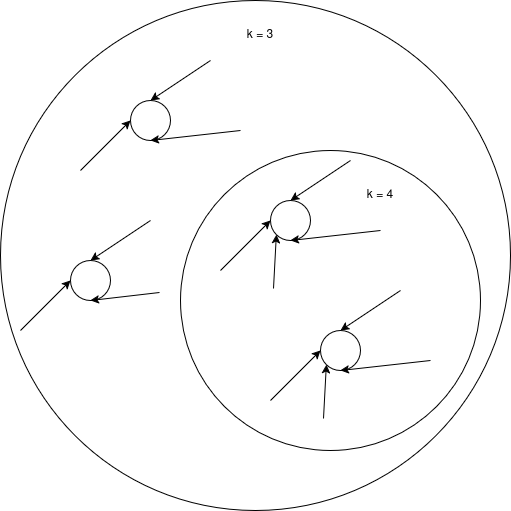
\includegraphics[width=0.5\textwidth]{images/powerLaw.png}
        \caption{$A_t(k + 1) \subseteq A_t(k)$}
\end{figure}

 Per definizione, il nodo $j \in A_t(k) \iff j \leq t\ \land\ x_j(t) \geq k$. Espandendo la seconda condizione, abbiamo che:
\begin{align*}
x_j(t) &= \frac{p}{1-p}\left[\left( \frac{1}{j}\right)^{1-p} - 1\right] \geq k \\
&\iff \left( \frac{1}{j}\right)^{1-p} \geq \frac{1-p}{p}k + 1 \\
&\iff \left( \frac{1}{j}\right) \geq \left[\frac{1-p}{p}k + 1\right]^{\frac{1}{1-p}} \\
&\iff j \leq t\left[\frac{1-p}{p}k + 1\right]^{-\frac{1}{1-p}}
\end{align*}
Osserviamo adesso che 
\[
\left.
\begin{aligned}
& \frac{1-p}{p}k + 1 > 1 \\
& -\frac{1}{1-p} < 0
\end{aligned}
\right\}
\;\Rightarrow\;
\left[\frac{1-p}{p}k + 1\right]^{-\frac{1}{1-p}} < 1
\;\Rightarrow\; t\left[\frac{1-p}{p}k + 1\right]^{-\frac{1}{1-p}} < t
\]
In conclusione, 
\[
A_t(k) = \left\{j\ |\ j \leq t\left[\frac{1-p}{p}k + 1\right]^{-\frac{1}{1-p}}\right\}
\]
quindi,
\[
|A_t(k)| = t\left[\frac{1-p}{p}k + 1\right]^{-\frac{1}{1-p}}
\]
Riuscendo quindi a calcolare la dimensione dell'insieme $A_t(k)$. Con questo risultato, possiamo adesso calcolare quanto vale la frazione dei nodi con grado esattamente $k$ (il numero di nodi con grado almeno $k$ - il numero di nodi con grado almeno $k + 1$), ovvero:
\[
\frac{1}{t}[|A_t(k)| - |A_t(k+1)|]
\]
Per semplicità, definiamo:
\[
F(k) = \left[\frac{1-p}{p}k + 1\right]^{-\frac{1}{1-p}}
\]
ottenendo quindi,
\[
f(k) = F(k) - F(k + 1) = \frac{1}{t}[|A_t(k)| - |A_t(k+1)|]
\]
Poiché $f(k) = F(k) - F(k + 1)$, possiamo approssimarla con la sua derivata, ovvero, $f(k) \approx - \frac{dF(k)}{dk}$, quindi:
\[
\begin{aligned}
f(k) \approx - \frac{dF(k)}{dk} &= \frac{(1-p)}{p}\left[-\frac{1}{1-p}\right]\left[\frac{(1-p)}{p}k+1\right]^{-\frac{1}{1-p}-1}\\
&= \frac{1}{p}\left[\frac{(1-p)}{p}k+1\right]^{-\frac{1}{1-p}-1} 
\end{aligned}
\]
Che è una \textbf{Power Law} con esponente $1 + \frac{1}{1-p}$.
In conclusione, nel modello Rich Get Richer, con alta probabilità la frazione del numero di nodi di grado $k$ è proporzionale a 
\[k^{-\frac{1}{1-p}-1}.\]

\newpage

\section{Grafi Geometrici aleatori e reti wireless}

Fino adesso abbiamo parlato di modelli di generazione di grafi aleatori per reti virtuali. In questo capitolo ci focalizziamo invece sulle reti fisiche, nel dettaglio sulle reti wireless ad hoc.

Le reti wireless ad hoc sono composte da nodi dotati di ricetrasmettitori che comunicano in modalità peer-to-peer, spesso tramite percorsi multi-hop, cioè attraverso nodi intermedi che inoltrano i messaggi fino alla destinazione.  

Le reti di sensori rappresentano una particolare categoria di reti ad hoc, in cui ogni nodo include un sensore, una batteria a bassa capacità, un processore semplice e un modulo wireless. Questi nodi raccolgono e trasmettono dati ambientali (come temperatura o pressione), eventualmente comprimerli o aggregarli, per fornire una visione complessiva dell'area monitorata. I dati possono poi essere accessibili da utenti esterni tramite nodi gateway.  

Le applicazioni spaziano dal monitoraggio ambientale e meteorologico al controllo di infrastrutture e sistemi industriali.

Per garantire la comunicazione tra tutti i nodi di una rete, questa deve essere connessa: per ogni coppia di nodi deve esistere un percorso di collegamenti diretti (multi-hop) che permetta alle informazioni di viaggiare da uno all'altro.

\vspace{0.5cm}

\begin{definizione}[Grafo Geometrico]
    Un grafo geometrico G = \{V, E, r\} consiste in un insieme $V$ di nodi in uno spazio metrico ($\mathbb{R}^2$), dei quali conosciamo le coordinate, e un parametro $r > 0$. Quindi: 
    \begin{itemize}
        \item $V = \mathbb{R}^2$, quindi $\forall,\ A \in V,\ A = \{x_A, y_B\}$.
        \item $E = \{(A, B): A \in V \land B \in V \land \sqrt{(x_A - x_B)^2 + (y_A - y_B)^2} \leq r\}$
    \end{itemize}
\end{definizione}

Generalmente si normalizza per $r$, ossia si riportano i punti in scala $1:r$. In questo caso, quando $r = 1$, il grafo prende il nome di \textbf{Unit Disk Graph}.

\vspace{0.5cm}

\begin{definizione}[Grafo Geometrico Aleatorio]
    Siano $n \in \mathbb{N}$ e $0 < r \leq \sqrt{2}$. Un \textbf{grafo geometrico aleatorio} $G(n, r)$ è un particolare grafo geometrico, definito all'interno di un quadrato $Q = [0,1] \times [0, 1]$. In pratica vengono scelti uniformemente a random $n$ punti all'interno di $Q$.
\end{definizione}

La scelta che $0 < r \leq \sqrt{2}$ dipende appunto dal fatto che $Q$ è il quadrato unitario, la cui diagonale misura $\sqrt{2}$. Infatti:
\begin{itemize}
    \item $r = \sqrt{2}$, $G(n, \sqrt{2})$ è un grafo completo;
    \item $r = 0$, $G(n, 0)$ è un grafo costituito da soli nodi isolati.
    \item In generale, se $r \rightarrow 0$, il grafo diventa sempre più sparso, mentre se $r \rightarrow \sqrt{2}$, il grafo diventa sempre più completo.
\end{itemize}

Questo particolare modello può avere numerosi riscontri pratici.
Per esempio consideriamo una situazione in cui si hanno a disposizione $n$ sensori ambientali per l'acquisizione di dati utili allo studio di fenomeni atmosferici, e di doverli disporre in una vasta area di $10,\ km^2$. 
Prima di spargere i sensori è possibile impostare un raggio 
$r$ di trasmissione, utile ai sensori per scambiarsi informazioni. Ovviamente maggiore è il raggio di trasmissione  $r$, maggiore sarà il consumo di batteria dei sensori.
Questi sensori inoltre verranno rilasciati nell'ambiente in maniera casuale lanciandoli da un aereo che sorvolerà l'area.

L'obiettivo è ora trovare il più piccolo valore di $r = r(n)$ (in funzione di $n$) tale che, con buona probabilità, la rete $G(n, r(n))$ risulti sempre connessa al crescere di $n$.

\subsection{Reti Wireless ad-hoc}

Per contestualizzare meglio il problema che stiamo studiando, consideriamo le \textbf{reti wireless ad-hoc}.

Una rete wireless ad-hoc è costituita da un insieme di dispositivi, ad esempio calcolatori o sensori, dislocati in un area. Ciascun dispositivo è dotato di un ricetrasmettitore wireless e di una batteria di capacità limita.

Ciascun ricetrasmettitore può essere configurato affinché possa trasmettere entro un certo raggio, che prende il nome di raggio di trasmissione.
\begin{definizione}[Raggio di trasmissione]
    Il raggio di trasmissione $r_x$ di un trasmettitore $x$ è la distanza entro la quale il dispositivo può inviare/riceve messaggi.    
\end{definizione}

\vspace{0.5cm}

\begin{definizione}[Grafo di comunicazione]
    Ad una rete di comunicazione è associato un grafo diretto, chiamato grafo di comunicazione. I nodi di questo grafo sono sono i dispositivi della rete. Dati due dispositivi $x$ e $y$, allora esiste l'arco $(x, y) \iff d(x, y) \leq r_x$.
\end{definizione}

\begin{figure}[ht!]
    \centering
    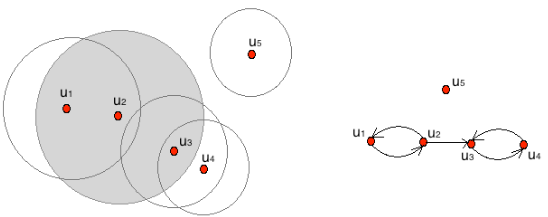
\includegraphics[width=0.5\linewidth]{images/grafo_comunicazione.png}
    \caption{Grafo di comunicazione}
    \label{fig:gc}
\end{figure}

Quindi, quando un nodo proverà a trasmettere ad un nodo che non rientra nel suo raggio di trasmissione, non potrà inviarlo direttamente ma dovrà utilizzare un percorso all'interno del grafo. Una comunicazione di questo tipo prende il nome di \textbf{comunicazione multi-hop}. Infatti, nella \autoref{fig:gc}, $u_1$ può inviare un messaggio a $u_4$ utilizzando il percorso $\{(u_1, u_2), (u_2, u_3),(u_3, u_4)\}$. Ovviamente, un nodo $x$ può inviare messaggi ad un nodo $y$ solo se esiste un percorso $x, \dots, y$ all'interno del grafo. 

 Perciò, se vogliamo che ciascun nodo possa comunicare con qualunque altro nodo è necessario che il grafo di comunicazione sia \textbf{fortemente connesso}. Questo problema si può risolvere facilmente impostando a ciascun nodo il raggio di trasmissione pari alla distanza di quel nodo dal nodo ad esso più distante, ovvero:

 Sia $V$ l'insieme dei nodi e sia $d(u, v)$ la distanza tra $u$ e $v$, allora,
\[
\forall\ u \in V,\ r_u = \max\{d(u, v):\ v \in V - \{u\}\}
\]

In questo modo, ciascun nodo può comunicare con qualunque altro nodo. Il problema è che l'energia che occorre ad un nodo per trasmettere i suoi messaggi è tanto maggiore quanto è più grande il raggio di trasmissione di quel nodo, perciò dobbiamo assegnare a ciascun nodo un raggio di trasmissione più piccolo.

 Riassumendo, possiamo modellare il problema descritto sopra nel seguente modo.
Assumiamo che tutti gli $n$ nodi abbiano lo stesso raggio di trasmissione $r(n)$. Inoltre, assumiamo che gli $n$ nodi siano distribuiti uniformemente a caso in un quadrato $Q = [0,1] \times [0, 1]$. La rete dunque è modellata da un grafo geometrico aleatorio $G(n, r(n))$, non orientato, in quanto $d(x, y) \leq r(n) \iff d(y, x) \leq r(n)$.

Il problema che dobbiamo studiare è:
\textbf{Dati $n$ punti distribuiti uniformemente a caso nel quadrato $Q = [0, 1] \times [0, 1]$ calcolare il valore minimo di $r(n)$ affinché $G(n, r(n))$ sia connesso}.

\subsection{Connessione di $G(n, r(n))$}

In questa sezione ci occuperemo di dimostrare la connettività di $G(n, r(n))$.

\begin{teorema}[Connessione di $G(n, r(n))$]
    Sia $r^*(n) = \min\{r(n)\}$ che garantisce, con probabilità ragionevole, che $G(n, r(n))$ è connesso, allora,
    \[
    r^*(n) \in \Theta\left(\sqrt{\frac{\ln n}{n}}\right)
    \]
\end{teorema}

Per mostrare la precedente affermazione è necessario dimostrare due teoremi che mostrano rispettivamente una \textbf{limitazione superiore ed una inferiore} per il minimo raggio di trasmissione $r^*(n)$.

\subsubsection{Delimitazione superiore al minimo raggio di connessione}

 \begin{teorema}[Delimitazione superiore al minimo raggio di connessione]
    Esiste una costante $\gamma_1 > 0$ tale che se $r(n) \geq \gamma_1 \left(\sqrt{\frac{\ln n}{n}}\right)$, allora $G(n, r(n))$ è connesso con \textbf{alta probabilità}.
\end{teorema}

\begin{proof}
    Sia $k(n) > 0$ un intero (dipendente da $n$). Partizioniamo $Q = [0, 1] \times [0, 1]$ in $k^2(n)$ celle, ciascuna di lato $\frac{1}{k(n)}$. Poniamo $r(n)$ pari alla lunghezza della diagonale di una coppia di celle adiacenti (due celle aventi un lato in comune), ovvero
    \[
    r(n) = \sqrt{\left(\frac{2}{k(n)}\right)^2 + \left(\frac{2}{k(n)}\right)^2} = \frac{\sqrt{5}}{k(n)}
    \]

\begin{figure}[ht!]
    \centering
    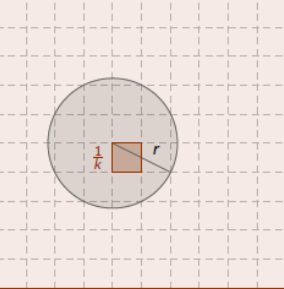
\includegraphics[width=0.3\linewidth]{images/delsup1.png}
    \label{fig:placeholder}
\end{figure}

 Ponendo $r(n) = \frac{\sqrt{5}}{k(n)}$, ciascun nodo in una qualsiasi cella è collegato da un arco a \textbf{tutti} i nodi (eventualmente) contenuti in tutte le celle adiacenti. Quindi se riuscissimo a dimostrare che con alta probabilità ciascuna cella contiene \textbf{almeno} un nodo, avremmo dimostrato che $G(n, r(n))$ è connesso con alta probabilità.

 \textbf{Dobbiamo quindi dimostrare che è possibile scegliere $k(n)$ in modo tale che, con alta probabilità, nessuna cella è vuota}.
Per calcolare questa probabilità, per semplicità consideriamo la probabilità complementare, ovvero che \textbf{esiste almeno una cella vuota}.

 Sia $C$ una cella, l'obbiettivo è trovare una \textbf{delimitazione superiore} alla probabilità che 
\[\Pr[C = \emptyset]\]
L'evento $C = \emptyset$ lo possiamo scrivere come intersezione di più eventi, ovvero
\[
C = \emptyset \iff 1 \notin C \land 2 \notin C \land \dots \land n \notin C = \bigcap_{1 \leq i \leq n}(i \notin C)
\]
Da cui segue
\[
\Pr[C = \emptyset] = \Pr\left[\bigcap_{1 \leq i \leq n}(i \notin C)\right]
\]
Poiché i nodi sono posizionati in $Q$ \textbf{indipendentemente} gli uni dagli altri
\[
\Pr\left[\bigcap_{1 \leq i \leq n}(i \notin C)\right] = \prod_{1 \leq i \leq n}\Pr(i \notin C)
\]
Dobbiamo ora capire quanto vale $\Pr(i \notin C) = 1 - \Pr(i \in C)$. La probabilità che il nodo $i$ sia scelto all'interno della cella $C$ è pari al rapporto fra l'area di $C$ e l'area del quadrato $Q = [0,1] \times [0,1]$. Quindi
\[
\Pr[i \in C] = \frac{Area_C}{Area_Q} = \frac{1}{k^2(n)}
\]
Da cui segue che
\[
\Pr(i \notin C) = 1 - \Pr(i \in C) = 1 - \frac{1}{k^2(n)}
\]
Quindi
\[
\Pr[C = \emptyset] = \Pr\left[\bigcap_{1 \leq i \leq n}(i \notin C)\right] = \prod_{1 \leq i \leq n}\Pr(i \notin C) = \left(1 - \frac{1}{k^2(n)}\right)^n
\]
Calcolata la probabilità che la cella $C$ sia vuota, si vuole ora calcolare la probabilità dell'evento che esista \textbf{almeno} una cella vuota, ovvero
\[
\Pr[\exists\ C: C = \emptyset] = \Pr\left[\bigcup_{C \in Q}(C = \emptyset)\right]
\]
Applicando la Union Bound\footnote{La Union Bound dice che la probabilità dell'unione di eventi è minore o uguale della somma delle loro probabilità}
\[
\Pr[\exists\ C: C = \emptyset] \leq \sum_{C \in Q}\Pr[C = \emptyset] \leq k^2(n)\left(1 - \frac{1}{k^2(n)}\right)^n
\]
Sostituendo $k(n) = \frac{\sqrt{5}}{r(n)}$, otteniamo che
\[
\Pr[\exists\ C: C = \emptyset] \leq \sum_{C \in Q}\Pr[C = \emptyset] \leq \frac{5}{r^2(n)}\left(1 - \frac{r^2(n)}{5}\right)^n
\]
A questo punto, poniamo $r(n) = \gamma_1\left(\sqrt{\frac{\ln n}{n}}\right)$ ottenendo,
\[
\Pr[\exists\ C: C = \emptyset] \leq \sum_{C \in Q}\Pr[C = \emptyset] \leq \frac{5n}{\gamma_1^2\ln n}\left(1 - \frac{\gamma_1^2\ln n}{5n}\right)^n
\]
Sapendo che $\forall x \in \mathbb{R},\ 1 - x \leq e^{-x}$ e inoltre, se $x \neq 0$, allora $1 - x < e^{-x}$.

 Poiché $\frac{\gamma_1^2\ln n}{5n} \neq 0$, per ogni $n \in \mathbb{N}$, otteniamo che
\[
\left(1 - \frac{\gamma_1^2\ln n}{5n}\right)^n < e^{-\frac{\gamma_1^2\ln n}{5n}}
\]
Quindi
\begin{align*}  
\Pr[\exists\ C: C = \emptyset] &< \frac{5n}{\gamma_1^2\ln n}e^{-\cancel{n}\frac{\gamma_1^2\ln n}{5\cancel{n}}} < \frac{5n}{\gamma_1^2}e^{-\frac{\gamma_1^2\ln n}{5}} \\
&= \frac{5n}{\gamma_1^2}n^{-\frac{\gamma_1^2}{5}} = \frac{5}{\gamma_1^2}n^{1 - \frac{\gamma_1^2}{5}}
\end{align*}
Poiché vogliamo che questa probabilità sia più piccola possibile, ovvero che
\[
\Pr[\exists\ C: C = \emptyset] < \frac{b}{n^c} \in \left(\frac{1}{n}\right)^{\Omega(1)}
\]
l'esponente $1 - \frac{\gamma_1^2}{5}$ deve essere negativo. Infatti, per $\gamma_1 > \sqrt{5},\ 1 - \frac{\gamma_1^2}{5} < 0$, quindi
con alta probabilità
\[
\Pr[G(n, r(n) \text{ è connesso })] \geq \Pr[\nexists\ C = \emptyset] = 1 - \Pr(\exists\ C: C = \emptyset) > 1 - \frac{b}{n^c} = 1 - \frac{5}{\gamma_1^2}n^{1 - \frac{\gamma_1^2}{5}} 
\]
In conclusione, abbiamo dimostrato che se $r(n) = \gamma_1\left(\sqrt{\frac{\ln n}{n}}\right)$ e $\gamma_1 > \sqrt{5}$, il grafo $G(n, r(n))$ è connesso con alta probabilità.
\end{proof}

\subsubsection{Delimitazione inferiore al minimo raggio di connessione}

\begin{osservazione}
    Nella prova della delimitazione superiore, ossia, che $r^*(n) \leq \gamma_1\left(\sqrt{\frac{\ln n}{n}}\right)$, abbiamo dovuto cercare una \textbf{maggiorazione} della probabilità che $G(n, r(n))$ è non connesso, ossia abbiamo dovuto dimostrare che $\Pr[G \text{ non connesso}] \leq \text{qualcosa}$.

     Ora, per dimostrare che $r^*(n) \geq \sqrt{\frac{\ln (n) + c}{n}}$, dobbiamo dimostrare una \textbf{minorazione} della probabilità che $G(n, r(n))$ è non connesso, ossi, dobbiamo dimostrare che $\Pr[G \text{ non connesso}] \geq \text{qualcosa}$.
\end{osservazione}

\begin{teorema}[Delimitazione inferiore al minimo raggio di connessione]
    Per ogni costatante $c > 0$, se $r(n) = \sqrt{\frac{\ln(n) + c}{n \pi}}$, allora 
    \[\lim_{n \rightarrow \infty} \Pr[G(n, r(n) \text{ è non connesso }] > 0
    \]
\end{teorema}

\begin{proof}
    Nel corso della dimostrazione, denoteremo con $G = G(n, r(n))$ e con $r = r(n)$. Come anticipato prima, dobbiamo trovare una \textbf{minorazione} per $\Pr[G \text{ non connesso}]$. Per iniziare, introduciamo i seguenti eventi:
    \begin{itemize}
        \item $\mathcal{E}_{\geq 1} = G$ contiene \textbf{almeno} un nodo isolato.
        \item $\mathcal{E}_{i_1, i_2, \dots, i_h} = $ tutti i nodi $i_1, i_2, \dots, i_h$ sono isolati in $G$, con $i_1, i_2, \dots, i_h \in [n]$.
        \item $\mathcal{E}_{i!} = i$ è l'unico nodo isolato in $G$, con $i \in [n]$.
    \end{itemize}

 Ai fini della dimostrazione, dobbiamo ricordare la seguente proposizione: 
 Dati due eventi $A$ e $B$, se $A \implies B$, allora
\[
    \Pr[A] \leq \Pr[B].    
\]

 Questo significa che ogni volta che accade $A$ accade anche $B$ (in termini insiemistici $A \subseteq B$). 
Ora, la probabilità è una \textbf{misura} (nel senso matematico): più grande è l'insieme, più grande (o uguale) è la sua probabilità, quindi
\begin{align}
A \subseteq B \implies \Pr[A] \leq \Pr[B]
\end{align}

 Ritornando alla nostra dimostrazione, possiamo fare le seguenti osservazione:
\begin{itemize}
    \item {
        se $G$ contiene almeno un nodo isolato allora $G$ è non connesso, ovvero
        \[
        \mathcal{E}_{\geq 1} \implies \text{G non connesso}
        \]
        Implica
        \[
        \Pr[\mathcal{E}_{\geq 1}] \leq \Pr[\text{G non connesso}]
        \]
    }
    \item {
        Inoltre, se accade che 1 è l'unico nodo isolato in $G$, oppure 2 è l'unico nodo isolato in $G$, oppure $\dots$, oppure $n$ è l'unico nodo isolato in $G$, allora accade che $G$ contiene un nodo isolato, formalmente, se
        \[
        \bigcup_{i \in [n]} \mathcal{E}_{i!} \implies \mathcal{E}_{\geq1}
        \]
        allora
        \[
        \Pr\left[\bigcup_{i \in [n]} \mathcal{E}_{i!}\right] \leq \Pr[\mathcal{E}_{\geq1}]
        \]
    }
\end{itemize}

In entrambi i casi, è stata applicata la $(1)$.

Poiché $\mathcal{E}_{1!}, \mathcal{E}_{2!}, \dots, \mathcal{E}_{n!}$ sono eventi disgiunti, allora
\[
\Pr\left[\bigcup_{i \in [n]} \mathcal{E}_{i!}\right] = \sum_{i \in [n]}\Pr[\mathcal{E}_{i!}]
\]

In conclusione, abbiamo trovato una \textbf{minorazione} per $\Pr[G \text{ non connesso}]$, ovvero
\[
\Pr[G \text{ non connesso}] \geq \sum_{i \in [n]}\Pr[\mathcal{E}_{i!}]
\]

 Non è, però, semplice calcolare direttamente $\Pr[\mathcal{E}_{i!}]$. Allora, dobbiamo trovare delle espressioni più facili per poterla minorare. Osserviamo che il nodo $i$ è l'unico isolato in $G$, se e solo se $i$ è un nodo isolato in $G$ e inoltre, comunque scegliamo un altro nodo $j$, $i$ e $j$ non sono entrambi isolati in $G$, ovvero
\[
\mathcal{E}_{i1} = \mathcal{E}_i \bigcap_{j \in [n] - \{i\}} \mathcal{E}_{ij}^C = \mathcal{E}_i - \bigcup_{j \in [n] - \{i\}}\mathcal{E}_{ij}
\]
Quindi,
\begin{align*}
    \Pr[\mathcal{E}_{i!}] 
    &= \Pr\!\left[\mathcal{E}_i \setminus 
        \bigcup_{j \in [n] \setminus \{i\}}\mathcal{E}_{ij}\right] \\[4pt]
    &\underbrace{\geq}_{(1)} 
        \Pr[\mathcal{E}_i] 
        - \Pr\!\left[\bigcup_{j \in [n] \setminus \{i\}}\mathcal{E}_{ij}\right] \\[6pt]
    &\underbrace{\geq}_{(2)} 
        \Pr[\mathcal{E}_i] 
        - \sum_{j \in [n] \setminus \{i\}}\Pr[\mathcal{E}_{ij}]
\end{align*}

\smallskip

\textbf{(1)} Disuguaglianza di sottrazione per insiemi: 
\[
P(A\setminus B) = P(A) - P(A\cap B) \ge P(A) - P(B)
\]
poiché \(P(A\cap B) \le P(B)\). \\[4pt]
\textbf{(2)} Union Bound (o disuguaglianza dell'unione): 
\[
P\!\left(\bigcup_i A_i\right) \le \sum_i P(A_i)
\]

 Ricapitolando, l'obbiettivo della dimostrazione è quindi calcolare una \textbf{minorazione} per $\Pr[G \text{ non connesso}]$. Fino adesso siamo arrivati ai seguenti risultati:
\begin{enumerate}
    \item $\Pr[G \text{ non connesso}] \geq \sum\limits_{i \in [n]}\Pr[\mathcal{E}_{i!}]$
    \item $\Pr[\mathcal{E}_{i!}] \geq \Pr[\mathcal{E}_i] - \sum\limits_{j \in [n] \setminus \{i\}} \Pr[\mathcal{E}_{ij}]$
\end{enumerate}

 A questo punto non ci resta che trovare \textbf{una minorazione per $\Pr[\mathcal{E}_i]$ e una maggiorazione per $\Pr[\mathcal{E}_{ij}]$}.

Prima di procedere, indichiamo per ogni $t \in Q$, $C_r{t}$ il cerchio di centro $t$ e raggio $r$. Inoltre, per ogni $i \in [n],\ t_i \in Q$ è il punto del quadrato nel quale è posizionato il nodo $i$ (in pratica dobbiamo distinguere fra il concetto astratto di nodo e la sua posizione fisica nel piano). 

\textbf{Minoriamo $\Pr[\mathcal{E}_i]$}. L'evento $\mathcal{E}_i$ si verifica se e solo se, una volta fissato $t_i$, nessun nodo $j \neq i$ è posizionato in $C_r(t_i)$.

Quindi, \textbf{fissato} $t_i$ e \textbf{fissato} $j \neq i$,
\[
\Pr[t_j \notin C_r(t_i)] = \frac{Area(Q - C_r(t_i))}{Area(Q)} \geq \frac{Area(Q) - Area(C_r(t))}{Area(Q)} \geq 1 - \pi r^2
\]
Vale il "$\geq$", perché $C_r(t_i)$ potrebbe non essere completamente contenuto in $Q$ (se $t_i$ è vicino al bordo di $Q$).

Allora, \textbf{fissato} $t_i$, 
\[
\Pr[\forall j \neq i: t_i \notin C_r(t_i)] \geq (1 - \pi r^2)^{n - 1}
\]
La precedente probabilità è relativa a un dato $t_i$ fissato. Ciò che serve a noi però è dare una stima per un qualsiasi $i$ . Però, visto che $t_i$ è scelto uniformemente a caso in un intervallo continuo, allora la funzione di densità della scelta u.a.r. in $Q$ sarà $f(t) = \frac{1}{Area(Q)} = 1$. Quindi, integrando su tutti i punti del quadrato $Q$, abbiamo che:
\[
\Pr[\mathcal{E}_i] \geq \int_{t_i \in Q} f(t_i)(1 - \pi r^2)^{n - 1} dt_i = \int_{t_i \in Q} (1 - \pi r^2)^{n - 1} dt_i = (1 - \pi r^2)^{n - 1}
\]
\end{proof}

La dimostrazione di tale teorema si ferma qui, se avrò voglia farò anche il resto :) .

\newpage

\section{Modello Small World}

Consideriamo l'esperimento dello psicologo statunitense Stanley Milgram (1967). In tale esperimento Milgram scelse una persona target che risiedeva dalla parte opposta degli Stati Uniti. Dopodiché inviò una serie di lettere ad un gruppo di persone con le seguenti informazioni e regole:
\begin{enumerate}
    \item nella lettera era specificato nome, indirizzo, occupazione e altre informazioni riguardo il target
    \item chi riceveva questa lettera doveva inoltrarla (ovvero inviare una sola copia) ad un'altra persona, che secondo lui si avvicinava di più al target. Era possibile inviare la lettera ad una persona solo se la si conosceva di prima persona.
\end{enumerate}
    
Al termine dell'esperimento Milgram osservò che circa un terzo delle lettere riuscirono ad arrivare al target, ma ancor più interessante che tutte arrivarono mediamente in 6 passi.

Questo esperimento suggerì due proprietà importanti delle reti sociali:
\begin{enumerate}
    \item  un'abbondanza di cammini brevi tra gli individui della rete, noto come fenomeno \textbf{Small World (o "Six Degrees of Separation")}.
    \item tali cammini potevano facilmente essere individuati dagli individui, che altro non conoscono della struttura della rete se non il loro vicinato ed una euristica che gli consenta di intuire i vicini più plausibili per i cammini. Questo è noto come fenomeno della navigabilità.
\end{enumerate}

Certamente un aiuto molto rilevante per la navigabilità è stata la presenza di alcune informazioni riguardo il target nella lettera (oltre il nome).

Per esempio se so che il target abita in un certa regione cercherò come prima cosa di inoltrare la lettera a una persona che geograficamente si avvicina. Ancora, se so che è abbastanza vicino a me e so anche che è un medico, certamente cercherò tra le mie conoscenze una persona che lavora (o che ha a che fare) con l'ambiente sanitario (è meno probabile che mi avvicini se inoltro la lettera a un contadino).

Invece, se avessi avuto solamente il nome del target senza essere in grado nemmeno di individuare la sua città, molto probabilmente la lettera sarebbe stata perduta.

Per quanto riguarda l'abbondanza di cammini brevi invece una possibile motivazione intuitiva è la seguente: supponiamo di conoscere in maniera diretta 100 persone, e che tali persone conoscono direttamente altre 100 persone. Allora con due "hop" posso raggiungere $100 \cdot 100 = 10000$ altre persone. E se a loro volta gli amici dei miei amici conoscono 100 perso, in tre "hop" potrò raggiungere altri $100 \cdot 100 \cdot 100 = 1000000$ persone, e così via... .

Purtroppo però questo ragionamento è inconsistente, in quanto si fa un'assunzione molto forte, ovvero che ogni proprio amico conosce altre 100 persone distinte. In un conteso reale è però poco plausibile questa proprietà: se sono amico stretto di due persone è molto probabile che prima o poi essi si conoscano e diventino a loro volta conoscenti.

Per esempio le reti di conoscenze dei social networks mostrano la presenza di una quantità elevata di triangoli tra gli individui, a conferma di quanto osservato. La caratteristica di una rete di avere molti triangoli è detta \textbf{chiusura triadica (triadic closure)}, la quale diminuisce di molto il numero di individui raggiungibili con percorsi brevi rispetto al modello con crescita esponenziale.
\begin{figure}[ht!]
    \centering
    \begin{subfigure}[b]{0.45\linewidth}
        \centering
        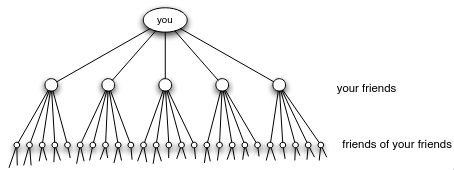
\includegraphics[width=\linewidth]{images/SMexp.png}
        \caption{\footnotesize Crescita puramente esponenziale delle conoscenze.}
    \end{subfigure}
    \hfill
    \begin{subfigure}[b]{0.45\linewidth}
        \centering
        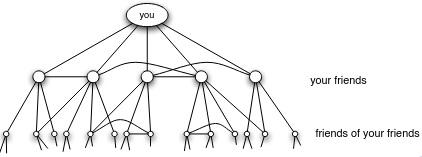
\includegraphics[width=\linewidth]{images/SMtriadic.png}
        \caption{\footnotesize La chiusura triadica diminuisce di molto il numero di persone raggiungibili con percorsi brevi.}
    \end{subfigure}
    \label{fig:sm_comparison}
\end{figure}

\subsection{Modello Watts - Strogatz}

Nel 1998 Duncan Watts and Steve Strogatz proposero un modello generativo di grafi aleatori che soddisfano due proprietà precedentemente viste: la presenza di numerosi triangoli e la presenza di cammini brevi che collegano le entità della rete.

Il grafo generato in accordo col modello Watts-Strogatz è composto da due componenti:
\begin{enumerate}
    \item una componente deterministica che consiste in una griglia bidimensionale
    \item una componente aleatoria sovrastante
\end{enumerate}

Il grafo fissato deterministicamente è una griglia "arricchita" - che corrisponde, sostanzialmente a uno Unit Disk Graph. I nodi sono considerati come punti in uno spazio metrico bidimensionale (un sottoinsieme di $\mathbb{N}^2$). Sono disposti sui punti a coordinate intere di un quadrato centrato nell'origine degli assi cartesiani e ogni nodo è collegato a ciascuno dei nodi vicini in orizzontale, verticale e diagonale.

\begin{definizione}[Griglia Arricchita]
    Fissato $n \in \mathbb{N}$. Un grafo a griglia "arricchita", è un grafo dove,    
    \begin{itemize}
        \item $V = \{(i, j) \in \mathbb{N}^2 : 0 \le i,j \le n \}$
        \item $E = \left\{ ((i,j),(a,b)) \in V^2 : [(a, b) = (i + \alpha,j + \beta): \alpha,\beta \in \{-1,0,1\}, (\alpha,\beta)\neq (0,0)]\right\}$
    \end{itemize}
\end{definizione}

Se si fa attenzione alla definizione di $E$ (ovvero l'insieme degli archi della componente deterministica), si può vedere che la griglia ha una sorta di \textit{periodicità}, ovvero i nodi a un bordo della griglia sono collegati ai nodi sul bordo opposto.
In questa maniera otteniamo un primo grafo con un'alta quantità di \textit{triangoli} (prima proprietà desiderata).

Per costruire la componente aleatoria fissiamo un $k>1$, e per ogni nodo $v \in V$ esso aggiungerà come ulteriori vicini altri $k$ nodi scelti \textbf{uniformemente a caso}.

\newpage

\begin{figure}[ht!]
    \centering
    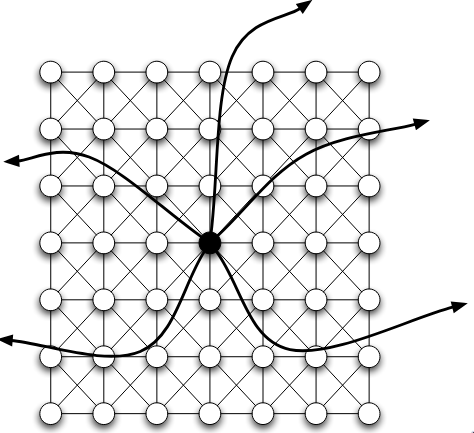
\includegraphics[width=0.5\linewidth]{images/SMWS.png}
    \caption{Watts-Strogatz}
\end{figure}

Come possiamo osservare, più che a una griglia su una superficie piana, dobbiamo pensare a \textbf{una griglia "appoggiata" su una superficie sferica}, che si racchiude su se stessa e che chiameremo \textbf{wrapped}.

Si può osservare una certa \textbf{dicotomia} tra gli archi deterministici e quelli aleatori:
\begin{enumerate}
    \item gli archi deterministici rappresentano un legame forte tra i nodi (\textbf{strong tie}), infatti tra due nodi legati da un arco deterministico esistono sempre dei triangoli. Possiamo dire che rappresentano delle relazioni "fisicamente" vicine.
    \item gli archi aleatori rappresentano invece delle conoscenze "alla lontana", e in quanto tale un legame debole (\textbf{weak tie}). Infatti è molto poco probabile trovare triangoli nella componente aleatoria (a meno che $k$ non sia molto grande).
\end{enumerate}

Ricapitolando, un grafo generato dal modello Watts-Strogatz contiene molti triangoli (\textbf{triadic closure}).
A questo punto rimane da chiederci se \textit{esistono numerosi cammini brevi tra i nodi della rete}.
Intuitivamente parlando, se si considerano cammini composti dai soli archi aleatori, è poco probabile incontrare due volte uno stesso nodo in brevi distanze. Successivamente \textit{Bollobàs e Ching} diedero una dimostrazione formale a questo fenomeno.
Più precisamente dimostrarono la presenza di cammini brevi in un modello con molta meno \textit{randomness}, individuando anche la lunghezza media degli shortest path nei grafi generati in accordo al modello di Watts-Strogatz. 

Consideriamo un nuovo modello simile a quello Watts-Strogatz, dove però solo un nodo su $k$ ha archi random, e il numero di archi random è pari a 1.
Partizioniamo poi la rete in "città" di $k \times k$ individui, e consideriamo il fenomeno small-world a livello di città.
Certamente ogni città avrà mediamente $k$ archi random, e inoltre ogni coppia di nodi $u,v$ di una stessa città sarà connessa da un cammino breve di lunghezza al più $2k$.

Venne dimostrato che per trovare un cammino relativamente corto tra due nodi $u,v$ di due città differenti, basta che $u$ raggiunga un nodo $w$ nella stessa città (in al più $2k$) passi, e poi tramite pochi salti passare da una città all'altra fino ad arrivare alla città di $v$.

In conclusione, anche con un piccolo ammontare di casualità, il modello Watts-Strogatz cattura il fenomeno "small-world".

\subsection{Navigabilità del modello Watts-Strogatz}

Supponiamo ora di essere il nodo $u$ in un grafo di Watts-Strogatz e vogliamo inviare un messaggio ad una certa destinazione $v$ \textbf{di cui conosciamo le coordinate}. Ovviamente, cerchiamo di fare arrivare il messaggio il più velocemente possibile, ossia cerchiamo di fare in modo che venga consegnato attraverso uno shortest path da $u$ a $v$. Poiché noi (nodo $u$) non conosciamo altro della rete se non i nostri vicini, facciamo tante copie del messaggio quanti sono i vicini e mandiamo una copia a ciascun vicino (al più 8/9 messaggi, numero costante). Ovviamente, potremmo procedere in modo diverso, ovvero potremmo scegliere, fra i nostri vicini quello le cui coordinate sono più prossime a quelle di $v$, ma la casualità dei weak ties potrebbe far si che, invece, un vicino che, al momento, mi appare peggiore ha un arco random che lo collega direttamente a $v$.

\begin{figure}[ht!]
    \centering
    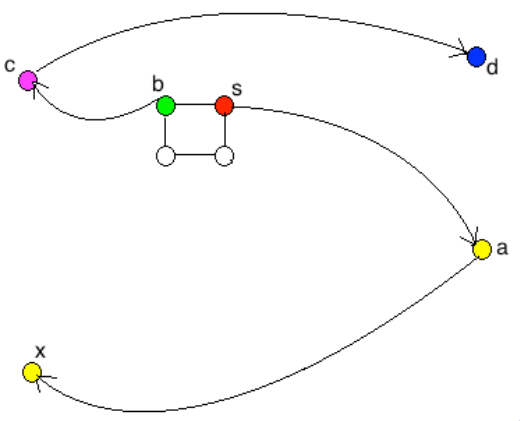
\includegraphics[width=0.5\linewidth]{images/SMexample.png}
    \caption{Esempio di navigabilità del grafo di WS}
    \label{fig:ex_navigabilità}
\end{figure}

Osservando la \autoref{fig:ex_navigabilità}, il nodo $s$ deve inviare un messaggio a $d$. Fra i vicini di $s$ il più vicino a $d$ \textbf{sulla griglia} è $a$, perché $b$ \textbf{sulla griglia} è più lontano di $a$ da $d$, e queste sono le uniche informazioni di cui $s$ è in possesso. Perciò, $s$ inoltra il messaggio ad $a$, che poi dovrà seguire i nodi della griglia per giungere a $d$. Supponiamo invece che $s$ avesse inoltrato il messaggio a $b$, in questo modo si sarebbe allontanato \textbf{sulla griglia} da $d$, ma avrebbe raggiunto $d$ in soli 3 passi, infatti il messaggio avrebbe seguito il percorso $s \rightarrow c \rightarrow a$ invece che $s \rightarrow a \rightarrow \dots \rightarrow d$.

Il nodo $u$ deve inviare un messaggio al nodo $v$. Per farlo, $u$ crea tante copie del messaggio quanti sono i suoi vicini, e ne invia una a ciascuno di essi.
Ciascun vicino, a sua volta, replica lo stesso comportamento: genera tante copie del messaggio quanti sono i propri vicini e le inoltra a tutti loro.
Il processo continua in questo modo iterativamente.
Dopo $h$ passi, nel grafo circolano $\approx 7^h$ copie del messaggio.
Questa procedura è nota come \textbf{flooding}. È evvidente che il numero di messaggio è inaccettabile, inoltre nel esperimento di Milgram, ad ogni passo circolavano tanti messaggi quanti ne aveva creati Milgram, e non aumentavano ad ogni passo (no \textbf{flooding}, eppure gli individui che parteciparono all'esperimento di Milgram avevano la stessa conoscenza dei nodi del modello di WS). Notiamo quindi, che il modello di WS non riesce a descrivere qualche caratteristica di una rete sociale che rende possibile la ricerca di Milgram.

\subsubsection{Ricerca decentralizzata (ricerca miope)}

Vogliamo un modo per trovare un cammino non troppo lungo tra $u$ e $v$ in modo da trasmettere una sola copia del messaggio, e non un numero esponenziale, un po' come fecero le persone che parteciparono all'esperimento di Milgram.

Purtroppo fare questo tipo di ricerca \textbf{miope} in un modello Watts -Strogatz non è possibile, e lo abbiamo visto negli esempi discussi sopra. Nell'esperimento di Milgram, gli individui coinvolti hanno utilizzato un algoritmo di ricerca decentralizzata, che in quel caso si dimostrava efficiente. Probabilmente, ad ogni passo, un individuo inoltrava la copia della lettera in suo possesso a quello fra i suoi contatti che stimava essere più vicino possibile al destinatario, dove "più vicino" può riferirsi a metriche diverse: più vicino geograficamente, o rispetto alla professione, a agli interessi culturali etc... .

Inoltre è stato anche dimostrato con questo tipo di ricerca (nota come \textbf{ricerca decentralizzata}), non solo non c'è nessuna garanzia di trovare un cammino corto, ma mediamente i cammini trovati sono molto più lunghi dei cammini minimi che esistono tra mittente e destinatario.

Sostanzialmente il problema è che gli archi random della componente aleatoria sono "troppo" casuali per dare un supporto alla ricerca decentralizzata.
Infatti in un contesto sociale reale, è molto poco probabile che due persone totalmente a caso entrino in contatto.

È invece più probabile avere archi casuali tra persone più vicine fisicamente, anziché tra persone molto lontane.

Quindi possiamo dire che questo modello non è navigabile, e quindi non rispecchia le caratteristiche volute.

\subsection{Un modello per la ricerca decentralizzata}

Vogliamo ora definire un modello generativo cui corrispondano grafi che contengono molti triangoli e nei quali esistono shortest paths fra le coppie di e nei quali \textbf{trovare gli shortest path mediante ricerca decentralizzata sia possibile}. Il nuovo modello è ancora basato sul grafo a griglia arricchita del modello WS, ma ora la probabilità che l'arco random uscente dal nodo $u$ sia $(u, v)$ è inversamente proporzionale alla distanza \textbf{sulla griglia} dei nodi $u$ e $v$, quindi
\[
\Pr[(u, v) \in E] = \frac{1}{Z_u} \frac{1}{d(u, v)^q}
\]
dove $d(u, v)$ indica la lunghezza di uno shortest path fra $u$ e $v$ \textbf{sulla griglia} (percorso che non contiene archi random), mentre $Z_u$ è un fattore di normalizzazione.

Poiché da ogni nodo deve uscire uno e un solo arco random, deve valere che:
Fissato un nodo $u \in V$, si assume che esso scelga un nodo $v \in V - \{u\}$ a cui connettersi in modo equiprobabile. Di conseguenza, la probabilità che esista un arco $(u,v)$ è la stessa per tutti i nodi $v \neq u$, e la somma di tali probabilità è pari a 1.

\begin{align*}
&\sum_{v \in V - \{u\}} \Pr[(u, v) \in E] 
    = \sum_{v \in V - \{u\}} \frac{1}{Z_u} \frac{1}{d(u, v)^q} = 1 \\
&\implies\quad 
Z_u = \sum_{v \in V - \{u\}} \frac{1}{d(u, v)^q}
\end{align*}

In pratica, poiché la griglia è simmetrica, allora $Z_u$ ha lo stesso valore per tutti i nodi e, pertanto, indicheremo il fattore di normalizzazione, semplicemente, come $Z$.

Il parametro $q$ invece prende il nome di \textbf{esponente di clustering}. Con $q = 0$, otteniamo il modello di WS. In generale, gli archi random sono "troppo random" quando $q$ è piccolo, "non abbastanza random" quando $q$ è grande. Ovviamente, la ricerca decentralizzata funziona meglo con alcune scelte di $q$ e peggio con altre. Quello che vogliamo ora mostrare è che esiste una scelta di $q$ che rende efficiente la ricerca decentralizzata, ossia, permette di trovare percorsi la cui lunghezza non è troppo lontana da quella
degli shortest paths.

È possibile però dimostrare, che data una griglia $d$-dimensionale wrapped, allora il componente di clustering ottimale sarà esattamente $q = d$.

Cerchiamo ora di dare una spiegazione intuitiva a questo fenomeno.
Riconsideriamo nuovamente l'esperimento di Milgram, dove però abbiamo il mittente $A$ che vive negli Stati Uniti mentre il destinatario $B$ vive a Roma quartiere Garbatella.
Certamente la prima cosa che farebbe $A$ sarebbe quella di inviare la lettera quantomeno ad una persona che vive in Europa.
Anche se $A$ non ha amici diretti in Europa a cui inviare la lettera, passandola ad altri amici negli USA troverà brevemente qualcuno che ha amici che vivono oltre oceano.
Per semplicità assumiamo che $A$ invii direttamente la lettera ad un suo amico $C$ che vive a Mosca.
A sua volta $C$ cerca tra i suoi amici qualcuno che abiti almeno in Europa Occidentale.
Da $C$ la lettera passa a $D$ che vive a Parigi.
Per fortuna $D$ ha un amico in Italia che però vive a Perugia, e quindi la lettera finisce in Umbria. $D$ si ricorda di avere un lontano parente $E$ nel Lazio, a cui invia la lettera.
Dopodiché $E$ invia la lettera ad un suo collega $F$ che abita a Roma Centocelle, il quale a sua volta invierà la lettera a un amico $G$ che abita a Garbatella.
Di li, sicuramente in un numero non esagerato di passi la lettera arriva a $B$.
Come si può intuire, il processo di ricerca decentralizzata procede per \textbf{scale di risoluzione}. Infatti, anche se per pochi salti la lettera percorre relativamente poca distanza, presto farà un salto che riduce drasticamente la distanza con la destinazione.

\begin{teorema}[Informale: Coefficiente di clustering ottimale per $d = 2$]
    Se la componente deterministica del grafo è una griglia bidimensionale $(d = 2)$, allora l'esponente di clustering ottimale è $q = 2$.
\end{teorema}
\begin{proof}
    Fissiamo un nodo $u$, e partizioniamo gli altri nodi in “anelli” concentrici intorno a $u$, in modo che la distanza cresca esponenzialmente.  
    In particolare, consideriamo i nodi con distanza da $u$ nell'intervallo:
    \[
    [2^h, 2^{h+1}), \quad h = 0, 1, 2, \dots
    \]
    
    Dato che i punti su una circonferenza crescono come il quadrato del raggio, il numero di nodi nell'intervallo $[2^h, 2^{h+1})$ sarà proporzionale a $2^{2h}$. Definiamo:
    \[
    A_h = \{x : 2^h \leq d(u,x) < 2^{h+1}\} \implies |A_h| = \pi (2^{h+1})^2 - \pi (2^h)^2 = 3 \pi 2^{2h}.
    \]
    
    Ora, la probabilità che un nodo $v$ a distanza $r \approx 2^h$ venga scelto come destinazione di un arco casuale da $u$ è:
    \[
    \Pr[v \text{ scelto}] \approx \frac{1}{d(u,v)^q} \approx 2^{-hq}.
    \]
    
    Di conseguenza, la probabilità che l'arco casuale cada in un blocco $A_h$ è:
    \[
    \Pr[A_h] \approx |A_h| \cdot 2^{-hq} \approx 2^{2h} \cdot 2^{-hq} = 2^{(2-q)h}.
    \]
    
    Vediamo cosa succede per diversi valori di $q$:
    \renewcommand{\arraystretch}{1.5}
    \begin{table}[h!]
    \centering
    \begin{tabular}{|c|c|c|}
    \hline
    \textbf{Valore di $q$} & $P(A_h) \approx 2^{(2-q)h}$ & \textbf{Significato} \\
    \hline
    $q < 2$ & $P(A_h)$ \textbf{aumenta} con $h$ & troppi archi lunghi \\
    \hline
    $q > 2$ & $P(A_h)$ \textbf{diminuisce} con $h$ & troppi archi corti \\
    \hline
    $q = 2$ & $P(A_h) \approx 2^{(2-2)h} = 2^0 = 1$ & \textbf{indipendente da $h$} \\
    \hline
    \end{tabular}
    \caption{Comportamento della probabilità $P(A_h)$ in funzione del parametro $q$}
    \end{table}
    
    Da questa analisi si vede che il valore ottimale è $q = 2$, poiché la probabilità $\Pr[A_h]$ risulta uniforme su tutti gli anelli, evitando sia archi troppo lunghi che troppo corti.
\end{proof}

Quindi, \textbf{i weak ties sono distribuiti uniformemente su tutte le scale di risoluzione}, e questo fa sì che, anche se per un certo numero di passi occorre utilizzare gli archi della griglia (perché gli archi random che si incontrano fanno allontanare dall'obiettivo, e, dunque, ad ognuno di questi passi ci si avvicina solo di un'inezia all'obiettivo) non occorreranno molti passi prima di arrivare ad un nodo il cui arco random diminuisce \textbf{drasticamente} la distanza dall'obiettivo (di un ordine di grandezza!).

\subsubsection{Prestazioni della ricerca miope (decentralizzata)}

Nella precedente sezione abbiamo dato un'idea intuitiva del perché una distribuzione inversamente quadratica dei weak ties rispetto alle distanze rende la ricerca decentralizzata possibile.

Per semplicità verrà fatta un'analisi rigorosa (e non intuitiva) di questo fenomeno su una griglia 1-dimensionale, ovvero un anello.

\begin{figure}[ht!]
    \centering
    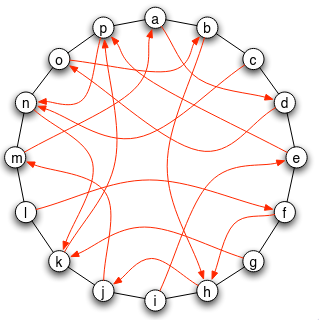
\includegraphics[width=0.3\linewidth]{images/SManello.png}
    \caption{Anello con random links}
\end{figure}

Consideriamo un grafo $G$ tale che:
\begin{itemize}
    \item $V = [n]$
    \item $E_d = \{(i, i+1) \in V: 1 \leq i < n\ \cup\ \{n, 1\}\}$, rappresentando la componente deterministica di partenza.
\end{itemize}
Quindi, in finale
\[
E = E_d \cup \left\{(u,v) \in V: \Pr[(u, v) \in E] = \frac{1}{Z} \frac{1}{d(u, v)}\right\}
\]
Sapendo quindi che $q = 1$, allora per ogni $u \in V$
\[
Z = \sum_{v \in V - \{u\}}\frac{1}{d(u, v)} \underbrace{=}_{(1)} 2 \sum_{1 \leq h \leq \frac{n}{2}} \frac{1}{h} \leq 2 \sum_{h = 1}^{\infty}\frac{1}{h} = 2 \ln n 
\]
\[
\implies Z \leq 2 \ln n
\]

Vale la \textbf{(1)} perché in un anello, il nodo $u$ ha due vicini a distanza 1, due vicini a distanza 3, e cosi via... .

\begin{osservazione}[Fasi dell'algoritmo]\label{oss:fasi}
    
Scegliamo uniformemente a casa due nodi $s$ e $t$ in $G$ ed utilizziamo l'algoritmo di ricerca decentralizzata per calcolare un percorso da $s$ a $t$. Indichiamo con $X$ la variabile aleatoria che denota la lunghezza di tale percorso e sia $\mathbb{E}[X]$ la lunghezza media di tali cammini.
Considerando una ricerca miope da $s$ a $t$, diremo che essa si trova della fase $j$ se il messaggio si trova ad una distanza compresa tra $2^j$ e $2^{j+1}$ dal destinatario. Poiché la distanza tra due nodi nell'anello è al più $\frac{n}{2}$, allora il numero massimo di fasi è al più $\log_2n$. Possiamo scrivere $X$ come la somma delle v.a. $X_1, X_2, \dots, X_{\log_2}$ dove $X_i$ è la lunghezza complessiva del cammino lungo la fase $i$
\[
X = X_1 + X_2 + \dots + X_{\log_2}
\]

Per linearità avremo che
\[
\mathbb{E}\left[ X \right] = \mathbb{E}\left[ X_1 + X_2 + ... + X_{\log_2{n}} \right] = \mathbb{E}\left[ X_1 \right] +  \mathbb{E}\left[ X_2 \right] + ... +  \mathbb{E}\left[ X_{\log_2{n}} \right]
\]
\end{osservazione}

\begin{teorema}
    Sia $\mathbb{E}\left[ X \right]$ la lunghezza media dei cammini risultati dalla ricerca miope tra una qualsiasi coppia di nodi, allora 
    \[
    \mathbb{E}\left[ X \right] \in O(\log^2{n})
    \]
\end{teorema}
\begin{proof}
    Siano i nodi $s,\ t$ rispettivamente il nodo \textbf{mittente} e il nodo \textbf{destinatario}. Abbiamo partizionato i nodi in base a distanze dalla sorgente $t$ che si \textit{dimezzano}, ovvero abbiamo definito la fase $j$ in cui il messaggio appartiene a un nodo $u$ con distanza
\[
\frac{d(s,t)}{2^{j+1}} \leq d(u,t) < \frac{d(s,t)}{2^j}
\]

Ricordando che il numero di fasi è al più $\log_2n$, e per quanto visto nella \autoref{oss:fasi}, per dimostrare il teorema è, quindi sufficiente dimostrare che:
\[
\forall j,\ \mathbb{E}[X_j] \in O(\ln n).
\]

Supponiamo di trovarci nel nodo $v$ durante la fase $j$, allora
\[
\frac{d(s,t)}{2^{j+1}} \leq d(v,t) < \frac{d(s,t)}{2^j}
\]
La fase $j$, termina sicuramente se esiste un nodo $z$ tale che
\[
(v, z) \in E\ \land d(z, t) \leq \frac{d(v, t)}{2} \leq \frac{1}{2} \frac{d(s, t)}{2^j} = \frac{d(s, t)}{2^{j + 1}} 
\]
Ovvero, sicuramente esiste quel arco $(v, z)$ che ci permette di dimezzare la distanza, e quindi passare nella prossima fase. Quindi
\begin{align*}
\Pr[\text{fase $j$ termina}] &= \Pr\left[\exists z \in V: (v, z) \in E \land d(z, t) \leq \frac{d(s, t)}{2^{j + 1}}\right] \\
&\underbrace{\geq}_{(1)} \Pr\left[\exists z \in V: (v, z) \in E \land d(z, t) \leq \frac{d(z, t)}{2} \right] 
\end{align*}
Vale la \textbf{(1)}, in quanto potrebbe essere che $d(v, t) = \frac{d(s, t)}{2^j}$, in tal caso, esisterebbe un arco $(v, z)$ nell'anello, tale che $d(z, t) = d(v, t) - 1 < \frac{d(s, t)}{2^j}$, e tale arco farebbe certamente terminare la fase $j$, e tuttavia sarebbe $d(z, t) > \frac{d(v, t)}{2}$ \textbf{(DA CAPIRE)}.

Indichiamo con $I$, l'insieme dei nodi che distano da $t$ non più della metà di quanto $v$ dista da $t$, ovvero:
\[
I = \left\{ u \in V: d(u, t) \leq \frac{d(v,t)}{2} \right\}
\]
Allora, 
\setlength{\jot}{10pt} % aumenta lo spazio verticale tra le righe
\begin{align*}
&\Pr\left[\exists z \in V: (v, z) \in E \land d(z, t) \leq \frac{d(z, t)}{2} \right] = \Pr\left[\exists z \in I: (v, z) \in E\right]\\
&= \Pr[\exists z \in I: (v, z) \text{ è un arco dell'anello oppure è un arco random}] \\
&= \sum_{z \in I}\Pr[(v, z) \text{ è un arco dell'anello oppure è un arco random}] \\
&\geq \sum_{z \in I}\Pr[(v, z) \text{ è un arco random}] = \sum_{z \in I}\frac{1}{Z}\frac{1}{d(v, z)}
\end{align*}
Dobbiamo ora stimare quanto vale $d(v, z)$. Certamente $v$ può raggiungere $z$ tramite un cammino del tipo $v \rightarrow t \rightarrow z$, e questo cammino sarà almeno lungo $d(v, z)$.
\[
d(v, z) \leq d(v, t) + d(t, z) = d(v, t) + d(z, t) \leq d(v, t) + \frac{d(v, t)}{2} = \frac{3d(v, t)}{2}
\]
Allora, per ogni $z \in I$,
\begin{align*}
    \sum_{z \in I}\Pr[(v, z) \text{ è un arco random}] &= \sum_{z \in I}\frac{1}{Z}\frac{1}{d(v, z)} \\ &\geq \sum_{z \in I} \frac{1}{Z}\frac{2}{3d(v, t)} \\ &\geq \sum_{z \in I}\frac{1}{2\ln n} \frac{2}{3d(v, t)} \\ &= \sum_{z \in I}\frac{1}{3d(v, t) \ln n} \\
    &= \frac{1}{3d(v, t)\ln n} |I|
\end{align*}

Dunque,
\[
\Pr\left[\exists z \in V: (v, z) \in E \land d(z, t) \leq \frac{d(z, t)}{2} \right] \geq \frac{1}{3d(v, t)\ln n} |I|
\]


Resta da valutare quanto vale $|I| = \left|\left\{ u \in V: d(u, t) \leq \frac{d(v, t)}{2} \right\}\right|$. 
Siano $v_{sin}$ e $v_{des}$ i due nodi in $I$ a distanza massima da $t$. Allora,

\[
d(v_{sin}, t) = d(v_{des}, t) = \left\lfloor\frac{d(v, t)}{2}\right\rfloor
\]

\begin{figure}[ht!] \centering 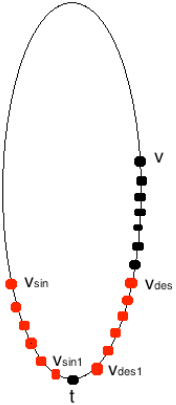
\includegraphics[width=0.2\linewidth]{images/Vsin_Vdes.png} \end{figure}


Ci prendiamo la parte intera inferiore, perché $\frac{d(v, t)}{2}$ potrebbe non essere intero. 
Siano ora $v_{sin_1}$ e $v_{des_1}$ i due nodi adiacenti a $t$. 
Allora $I$ contiene:
\begin{enumerate}
    \item Il nodo $t$
    \item gli $\left\lfloor\frac{d(v, t)}{2}\right\rfloor$ nodi da $v_{sin}$ a $v_{sin_1}$
    \item gli $\left\lfloor\frac{d(v, t)}{2}\right\rfloor$ nodi da $v_{des}$ a $v_{des_1}$
\end{enumerate}
Quindi,
\[
|I| = 1 + \left\lfloor\frac{d(v, t)}{2}\right\rfloor + \left\lfloor\frac{d(v, t)}{2}\right\rfloor 
\geq 1 + \frac{d(v, t) - 1}{2} + \frac{d(v, t) - 1}{2} = d(v, t)
\]

Riassumendo, l'obiettivo è di dimostrare che $\forall\ j,\ \mathbb{E}[X_j] \in O(\ln n)$.
Abbiamo ottenuto che 
\[
\Pr[\text{fase $j$ termina}] \geq \frac{1}{3d(v, t)\ln n} d(v, t) = \frac{1}{3 \ln n} 
\]
Quindi, 
\[
\Pr[\text{fase $j$ non termina}] \leq 1 - \frac{1}{3 \ln n}
\]
Quindi, la probabilità che non termini in $h$ passi è:
\[
\Pr[X_j \geq h] = \Pr[\text{fase $j$ \textbf{non} termina per $h$ passi}] \leq \left[1 - \frac{1}{3 \ln n}\right]^h 
\]

Per concludere, non resta che calcolare che $\mathbb{E}[X_j]$.
\begin{align*}
\mathbb{E}[X_j] &= 1 \cdot \Pr[X_j = 1] + 2 \cdot \Pr[X_j = 2] + \dots + \frac{n}{2} \cdot \Pr[X_j = \underbrace{\frac{n}{2}}_{d(s, t) \leq \frac{n}{2}}] \\
&= \Pr[X_j \geq 1] + 1 \cdot \Pr[X_j = 2] + \dots + (\frac{n}{2} - 1) \cdot \Pr[X_j = \frac{n}{2}] \\
&= \Pr[X_j \geq 1] + \Pr[X_j \geq 2] + 1 \cdot \Pr[X_j = 3] \dots + (\frac{n}{2} - 2) \cdot \Pr[X_j = \frac{n}{2}] \\
&=\dots \\
&= \sum_{1 \leq h \leq \frac{n}{2}} \Pr[X_j \geq h]
\end{align*}

A questo punto, abbiamo che
\begin{align*}
\mathbb{E}[X_j] &= \sum_{1 \leq h \leq \frac{n}{2}} \Pr[X_j \geq h] \leq \sum_{1 \leq h \leq \frac{n}{2}} \left[1 - \frac{1}{3 \ln n}\right]^h \\
& \leq \sum_{h \geq 0} \left[1 - \frac{1}{3 \ln n}\right]^h \underbrace{=}_{(1)} \frac{1}{1 - \left[1 - \frac{1}{3 \ln n}\right]} = 3 \ln n \\
\end{align*}
Vale la \textbf{(1)}, perché è stata riconosciuta una serie geometrica di ragione $q = \left[1 - \frac{1}{3 \ln n}\right]$, ricordando che la serie geometrica vale:
\[
\sum_{n = 0}^{\infty} q^n = \frac{1}{1 - q}
\]
Per concludere la dimostrazione, abbiamo che
\[
\mathbb{E}[X] = \sum_{1 \leq j \leq \log_2n} E[X_j] \leq \sum_{1 \leq j \leq \log_2n} 3 \ln n = \log_2 n \cdot 3 \ln n = \log_2 e \cdot \ln n \cdot 3 \ln n \in O(\ln^2 n) 
\]
\end{proof}

\newpage
\subsubsection{Perché $q = d$ funziona bene in $\mathbb{R}^d$}

Nel modello di Kleinberg, i nodi sono disposti su una griglia $d$-dimensionale, e ogni nodo $v$ è connesso:
\begin{itemize}
    \item ai \textit{vicini locali}, cioè ai nodi adiacenti nella griglia;
    \item a uno o più \textit{collegamenti di lungo raggio}, scelti con probabilità proporzionale a $\frac{1}{d(v,u)^q}$.
\end{itemize}

Il parametro $q$ controlla quanto le connessioni siano locali o globali: per $q$ piccolo, prevalgono archi lunghi; per $q$ grande, la rete è quasi regolare. L'obiettivo è capire per quale valore di $q$ la \textit{ricerca decentralizzata} (greedy routing) risulta efficiente, cioè richiede un numero di passi polilogaritmico per raggiungere una destinazione $t$.

In un anello, il numero di nodi entro distanza $d(v,t)$ è $|I| \approx d(v,t)$, mentre il fattore di normalizzazione è
\[
Z = \sum_{u \neq v} \frac{1}{d(v,u)} \le 2 \ln n.
\]
La probabilità che $v$ abbia un vicino $z$ tale che $d(z,t) \le \frac{d(v,t)}{2}$ è
\[
\Pr[\exists z: (v,z)\in E,\, d(z,t)\le\tfrac{d(v,t)}{2}] \ge \frac{1}{3\ln n},
\]
che è indipendente da $d(v,t)$. La ricerca può quindi procedere con una probabilità costante di avvicinarsi a $t$, risultando in un tempo atteso $O(\log^2 n)$.

In una griglia 2D, il numero di nodi entro distanza $d(v,t)$ cresce come l'area di un quadrato di lato $\approx d(v, t)$:
\[
|I| = \alpha\, d(v,t)^2,
\]
e il fattore di normalizzazione è
\[
Z = \sum_{u \neq v} \frac{1}{d(v,u)^2} \le \beta \ln n.
\]
Si ottiene così
\[
\Pr[\exists z: (v,z)\in E,\, d(z,t)\le\tfrac{d(v,t)}{2}] 
\ge \frac{4\alpha}{9\beta\ln n},
\]
ancora una volta indipendente da $d(v,t)$, e quindi la ricerca rimane efficiente.

In generale, in $\mathbb{R}^d$ la ricerca decentralizzata è efficiente se e solo se $q = d$.  
Solo in questo caso, il numero di nodi a distanza $\le d(v,t)$ cresce come $d(v,t)^d$ e il fattore di normalizzazione $Z$ cresce come $\ln n$, bilanciando perfettamente collegamenti locali e globali.  

Se $q < d$, le connessioni lunghe sono troppo frequenti e la rete perde struttura;  
se $q > d$, le connessioni sono troppo locali e la ricerca diventa lenta.  
Per $q = d$, invece, la rete è \textbf{navigabile}: mantiene la proprietà di small-world e consente una ricerca efficiente e decentralizzata.

\newpage
\subsubsection{Perché $q \neq d$ funziona male in $\mathbb{R}^d$}

Consideriamo il caso unidimensionale ($d = 1$) con $q = 0$. In questo scenario, la probabilità di scegliere un arco random $(u,v)$ è uniforme:
\[
\mathcal{P}((u,v) \in E) = \frac{1}{Z}\frac{1}{d(u,v)^0} = \frac{1}{Z}, \quad \text{dove} \quad Z = \sum_{v \neq u}\frac{1}{d(u,v)^0} = n - 1.
\]
Quindi, ogni arco random compare con probabilità $\frac{1}{n-1} > \frac{1}{n}$.

Definiamo ora l'insieme dei nodi entro distanza al più $\sqrt{n}$ dal destinatario $t$:
\[
R = \{ x \in V : d(x,t) \leq \sqrt{n} \}.
\]
Per un nodo $u \notin R$, la probabilità di connettersi tramite un arco random a un nodo di $R$ è:
\[
\Pr[\exists (u,v) \in E : v \in R] = \sum_{v \in R} \frac{1}{n} = \frac{|R|}{n} = \frac{2}{\sqrt{n}}.
\]

Sia $Y$ la variabile aleatoria che indica il numero di passi necessari per raggiungere $R$ partendo da $u$. Si ha:
\[
\Pr[Y \geq h] < \left(1 - \frac{2}{\sqrt{n}}\right)^h,
\quad
\mathbb{E}[Y] \leq \frac{1}{1 - \left(1 - \frac{2}{\sqrt{n}}\right)} = \frac{\sqrt{n}}{2}.
\]
Questo valore è già esponenzialmente più grande rispetto al tempo di ricerca miope nel caso $q=1$.

Per $q > 1$, gli archi random diventano più corti e la ricerca non migliora; per $q$ molto grande, la rete tende a ridursi alla sola componente deterministica.

\begin{teorema}
Sia $X$ la variabile aleatoria che rappresenta la lunghezza del cammino trovato dalla ricerca miope su un anello di $n$ nodi.  
Per ogni $q \neq 1$ esistono costanti $\alpha_q, c_q > 0$ tali che:
\[
\mathbb{E}[X] \geq \alpha_q \cdot n^{c_q}.
\]
\end{teorema}

Questi risultati, dimostrati per $d=1$, si estendono a dimensioni maggiori $d > 1$ con argomentazioni analoghe ma più complesse.
